For each query, provide a title, a description of what the query is supposed to
do, the (text of the) query, and a screenshot/table representing the (possibly
partial) outcome.

\section{Neo4j}

\subsection{Queries}
\begin{enumerate}
    \item \textbf{Mix \& Max}\\
This query analyzes recipes based on a provided list of ingredients to identify additional ingredients that frequently appear in combination with those in the list. It evaluates these additional ingredients by calculating their compatibility with the provided ingredients and their relevance based on recipe popularity and quality.
This query is particularly useful for recommending new ingredients to optimize the user's shopping list, suggesting new ingredients 
Key Steps and Functionality:
\begin{itemize}
    \item Input Ingredients:
The query uses a parameter, \$providedIngredients, which is a list of ingredients provided by the user.
    \item The query finds recipes (r) that contain at least one of the provided ingredients (i) and identifies other ingredients (i1) in those recipes that are not in the provided list. It ensures that these ingredients are distinct and tracks the count of how many provided ingredients are present in each recipe as availableMatchedIngredients.
    \item Calculate Average Recipe Rating:
For each matched recipe, the query retrieves associated reviews (rev) and calculates the average rating (avgRating) of those recipes.
    \item Aggregate Statistics for Matched Ingredients:
It counts the number of unique recipes (recipeCount) that include the matched ingredient (i1) in combination with the provided ingredients.
It computes the average of the average ratings (avgOfAvgRatings) across all recipes containing the matched ingredient.
It calculates the average number of provided ingredients matched in the recipes that contain the additional ingredient (IngredientCompatibility).
    \item Order Results by Relevance:
The results are ordered based on a relevance score that considers both the compatibility of the matched ingredient (IngredientCompatibility) and the logarithm of the number of recipes (log10(recipeCount)) where it is found. This ensures a balance between ingredient synergy and recipe popularity.
\end{itemize}

\subsubsection{Query}

\begin{minted}[frame=single, style=tango, fontfamily=lmss, breaklines]{cypher}
WITH $providedIngredients AS ingredients
MATCH (i:Ingredient)<-[:CONTAINS]-(r:Recipe)-[:CONTAINS]->(i1:Ingredient)
WHERE i.name IN ingredients AND NOT i1.name IN ingredients
WITH DISTINCT r, i1.name AS matchedIngredient, ingredients, COUNT(distinct i) as availableMatchedIngredients
MATCH (r)<-[:FOR]-(rev:Review)
WITH matchedIngredient, r, AVG(rev.rating) AS avgRating, ingredients, availableMatchedIngredients
MATCH (r)-[:CONTAINS]->(i:Ingredient)
WHERE i.name IN ingredients
RETURN matchedIngredient, COUNT(DISTINCT r) AS recipeCount, ROUND(AVG(avgRating),2) AS Rating, ROUND(AVG(availableMatchedIngredients),2) as Compatibility
ORDER BY Compatibility * log10(recipeCount) DESC;
\end{minted}

        
    \subsubsection{Results}
The results change based on what ingredients we put as a parameter. In this table the parameter \$providedIngredients is set as the list \begin{verbatim}['chicken', 'curry']\end{verbatim}
    \begin{table}[h!]
\centering
\begin{tabular}{lcccc}
\toprule
\textbf{Matched Ingredient} & \textbf{Recipe Count} & \textbf{Rating} & \textbf{Compatibility} \\
\midrule
Salt & 23 & 4.43 & 1.08 \\
Onion & 21 & 4.44 & 1.09 \\
Water & 14 & 4.38 & 1.13 \\
Garlic Cloves & 11 & 4.48 & 1.17 \\
Pepper & 15 & 4.45 & 1.0 \\
Butter & 13 & 4.92 & 1.0 \\
Chicken Broth & 11 & 4.02 & 1.0 \\
Celery & 10 & 4.45 & 1.0 \\
Olive Oil & 9 & 4.22 & 1.0 \\
Garlic Clove & 8 & 4.33 & 1.0 \\
Garlic & 7 & 3.79 & 1.0 \\
Lemon & 4 & 4.8 & 1.40 \\
Soy Sauce & 4 & 4.33 & 1.40 \\
Lemon Juice & 6 & 4.4 & 1.0 \\
Sugar & 6 & 4.17 & 1.0 \\
Mayonnaise & 5 & 4.20 & 1.0 \\
Flour & 5 & 4.65 & 1.0 \\
Milk & 5 & 4.61 & 1.0 \\
Carrots & 5 & 4.72 & 1.0 \\
Garlic Powder & 5 & 4.84 & 1.0 \\
\bottomrule
\end{tabular}
\caption{Mix \& Max}
\label{tab:ingredient_analysis}
\end{table}
    \clearpage
    \item \textbf{Recipe substitutes}\\
    This query suggests recipes that belong to the same category as a given recipe but have no shared ingredients, while maintaining a similar calorie count within a specified range.

Key Steps and Functionality:
    \begin{itemize}
        \item Find the Recipe Category:
The query starts by identifying the category (c) of a specified recipe (r1) using its name.
        \item Filter Recipes in the Same Category:
It retrieves other recipes (r2) that belong to the same category (c) but are not the same as the original recipe (r1).
        \item Calorie Range Matching:
Recipes are filtered to ensure their calorie count (r2.Calories) is within 100 calories of the specified recipe (r1.Calories).
The calorie values are handled using COALESCE to account for potential missing data.
        \item Exclude Shared Ingredients:
The query ensures no ingredients are shared between the original recipe (r1) and the suggested recipes (r2) by using a subquery that checks for the absence of overlapping Ingredient relationships.
        \item Sort by Calorie Difference:
Suggested recipes are ordered by the absolute difference in calories (CalorieDifference), ensuring the closest matches in terms of calorie content appear first.
    \end{itemize}
This query is useful for recommending alternative recipes within the same category that align with dietary preferences or calorie requirements, while ensuring a diverse ingredient selection.
            \subsubsection{Query}
            \begin{verbatim}
MATCH 
(r1:Recipe {Name: $recipeName })-[:BELONGS_TO]->(c:RecipeCategory)
<-[:BELONGS_TO]-(r2:Recipe)
WHERE 
ABS(COALESCE(r1.Calories, 0) - COALESCE(r2.Calories, 0)) <= 100 
AND r1 <> r2 
AND NOT EXISTS {
MATCH (r1)-[:CONTAINS]->(i:Ingredient)<-[:CONTAINS]-(r2)
}
RETURN 
r2.Name AS SimilarRecipe,
round(ABS(COALESCE(r1.Calories, 0) - COALESCE(r2.Calories, 0)), 1) 
AS CalorieDifference
ORDER BY 
CalorieDifference ASC;
            \end{verbatim}
        \subsubsection{Results}
    The results change based on what recipe name we put as a parameter. In this table the parameter \$recipeName is set as \begin{verbatim}'Mexican Lasagna'\end{verbatim}
        \begin{table}[h!]
\centering
\begin{tabular}{lc}
\toprule
\textbf{Similar Recipe} & \textbf{Calorie Difference} \\
\midrule
Big John's Stampede Chicken & 0.1 \\
Leek and Potato Pie & 0.7 \\
Tortellini With Roasted Eggplant \& Peppers-South Beach Diet & 0.8 \\
Birthday Caramel Chicken & 1.0 \\
Chicken and Vegi Stir Fry & 1.3 \\
Spinach Lasagna & 1.5 \\
Greek Chicken & 1.5 \\
Creamy Chicken Lasagna & 1.5 \\
Cuban Black Beans and Rice & 2.0 \\
Gang Bao Chicken & 2.1 \\
Chicken Etc. Risotto & 3.0 \\
Chicken Minestrone With Pesto & 3.0 \\
Oriental Beef & 3.3 \\
Stir-fried Noodles With Shrimp & 3.3 \\
Asparagus Risotto & 3.9 \\
Chicken Breasts Stuffed With Spinach and Mushrooms & 4.6 \\
Crumbled Hamburger (Sloppy Joes) & 4.6 \\
Chicken Pad Thai & 4.7 \\
Oatmeal Cottage Cheese Pancakes & 5.0 \\
Garden-Style Lasagna & 5.2 \\
\bottomrule
\end{tabular}
\caption{Recipe substitutes}
\label{tab:similar_recipes}
\end{table}
    \clearpage
    \item \textbf{Large groups meals}\\
    This query identifies recipes that require the least number of ingredients to prepare for a given number of servings, emphasizing recipes designed for large groups or higher servings.

Key Steps and Functionality:
\begin{itemize}
    \item - Filter Recipes Based on Serving Size:
    Recipes are selected based on their serving size (r.RecipeServings) or their association with categories and keywords indicating they are suitable for large groups:
    \begin{itemize}
        \item Recipes with servings greater than or equal to 10.
        \item Recipes belonging to the category For Large Groups or having the keyword For Large Groups.
    \end{itemize}
    \item Ingredient Collection: For each matching recipe, the query identifies all associated ingredients (i) and collects their names into a list (Ingredients). It counts the number of unique ingredients required for the recipe as RequiredIngredients.
    \item Sort by Ingredient Count:
Recipes are sorted in ascending order based on the number of ingredients required (RequiredIngredients), highlighting those that are simpler to prepare in terms of ingredient count.
    
\end{itemize}
This query is useful for users looking to prepare simple recipes with minimal ingredients, especially for large groups. It streamlines recipe selection by balancing simplicity and scalability.
        \subsubsection{Query}
        \begin{verbatim}
MATCH 
(c:RecipeCategory)<-[:BELONGS_TO]-(r:Recipe)-[:CONTAINS]->(i:Ingredient),
(r)-[:DESCRIBED_BY]->(k:Keyword)
WHERE 
tointeger(r.RecipeServings) >= 10 
OR c.name = 'For Large Groups' 
OR k.name = 'For Large Groups'
WITH 
r,
COLLECT(DISTINCT i.name) AS Ingredients,
COUNT(DISTINCT i) AS RequiredIngredients
RETURN 
r.Name AS RecipeName,
RequiredIngredients,
Ingredients
ORDER BY 
RequiredIngredients ASC;
        \end{verbatim}
        \subsubsection{Results}
        \begin{table}[h!]
\small % Reduce font size
\centering
\begin{tabularx}{\textwidth}{>{\raggedright\arraybackslash}Xc>{\raggedright\arraybackslash}X}
\toprule
\textbf{Recipe Name} & \textbf{Required Ingredients} & \textbf{Ingredients} \\
\midrule
Homemade Martinelli's & 1 & ["ginger ale"] \\
Lip-Smackin, Party-Snackin Mini Piggies in a Blanket & 1 & ["sharp cheddar cheese"] \\
Presto Pesto Rollups & 1 & ["pesto sauce"] \\
Cocktail Dogs & 1 & ["prepared mustard"] \\
Minty (Or Other Flavor) Chocolate Cookies & 1 & ["white chocolate bark"] \\
Toasted Baguette Slices & 1 & ["olive oil"] \\
Sweet Fire Jalapenos & 1 & ["sugar"] \\
Super Easy Peach Cobbler & 1 & ["butter"] \\
Cake Mix Cookies & 1 & ["eggs"] \\
Slow-Cooker Chocolate Pudding Cake & 1 & ["milk"] \\
Chocolate Pumpkin Muffins & 1 & ["pumpkin"] \\
Stained Glass Paint for Cookies & 1 & ["light corn syrup"] \\
Ranch Crackers & 1 & ["canola oil"] \\
OAMC Calzones & 1 & ["mozzarella cheese"] \\
Gorp & 1 & ["raisins"] \\
Cream Cheese Bacon Croissants & 1 & ["cream cheese"] \\
S'more Trail Mix Please! & 1 & ["miniature marshmallows"] \\
Cherry Glazed Smokies & 1 & ["ground black pepper"] \\
Muesli for Kids & 1 & ["papaya"] \\
Cocktail Party Meatballs & 1 & ["Heinz Chili Sauce"] \\
\bottomrule
\end{tabularx}
\caption{Recipes and Their Required Ingredients}
\label{tab:recipe_ingredients}
\end{table}

    \clearpage
    \item \textbf{Recipe suggestion for users}\\
This  query recommends recipes to a specific user based on the ingredients of recipes they have rated highly. It identifies recipes that share ingredients with these highly-rated recipes but that the user has not reviewed yet.

Key Steps and Functionality:
\begin{itemize}
    \item Identify High-Rated Recipes:
The query starts by finding recipes (r) reviewed by the user (u) with a high rating (rating > 4). It also identifies the ingredients (i) of these highly-rated recipes.
    \item Find Suggested Recipes:
It retrieves recipes (suggested) that contain one or more of the same ingredients as the user's high-rated recipes. It excludes recipes the user has already reviewed to ensure only new suggestions are presented.
    \item Ingredient Matching:
For each suggested recipe, the query counts the number of ingredients it shares with the user's high-rated recipes (matchingIngredients).
    \item Sort and Limit Results:
Suggested recipes are ordered in descending order based on the number of matching ingredients.
\end{itemize}

This query is particularly useful for personalized recipe recommendations. It leverages the user's past preferences to suggest recipes with similar ingredient profiles, ensuring relevance and increasing the likelihood of user satisfaction.
    
    \subsubsection{Query}
    \begin{verbatim}
MATCH 
(u:User)-[:WROTE]->(review:Review)-[:FOR]->(r:Recipe)
-[:CONTAINS]->(i:Ingredient)
WHERE 
review.rating > 4 AND u.name= $userName
MATCH 
(suggested:Recipe)-[:CONTAINS]->(i)
WHERE NOT
(u)-[:WROTE]->()-[:FOR]->(suggested)
WITH suggested, COUNT(DISTINCT i) AS matchingIngredients
RETURN 
suggested.Name AS recipeName,
matchingIngredients
ORDER BY 
matchingIngredients DESC;
    \end{verbatim}
    \subsubsection{Results}
The results change based on what user name we put as a parameter. In this table the parameter \$userName is set as \begin{verbatim}'Conan Lloyd'\end{verbatim}
    \begin{table}[h!]
\small % Reduce font size
\centering
\begin{tabularx}{\textwidth}{>{\raggedright\arraybackslash}Xc}
\toprule
\textbf{Recipe Name} & \textbf{Matching Ingredients} \\
\midrule
Crispy Chicken Tenders With Honey Mustard Sauce & 5 \\
Neely's Crispy Panko Chicken Tenders and Honey Mustard Sauce & 5 \\
Chicken Marsala & 5 \\
Red Lobster's Fried Soft-Shell Crab & 4 \\
Chicken Soup With Dumplings & 4 \\
Rocky Mountain Oysters & 4 \\
Vineyard Chicken & 4 \\
Chicken Pontalba & 4 \\
Creamy Ground Beef With Veggies and Pasta & 4 \\
Baked Chicken Nuggets & 4 \\
Company Chicken Pot Pie & 4 \\
Muenster Mushroom Chicken & 4 \\
Cheddar Cheese Cookies & 4 \\
Chicken With Cordon Bleu Gravy & 4 \\
Glazed Barbecued Ribs - Baked & 4 \\
Sarasota's Simple Sides-Mushrooms, Fennel, Tomatoes Onion & 4 \\
Tangy Beef Stroganoff & 4 \\
Ranch House Stew with Biscuit Crust & 4 \\
Broccoli Dijon & 4 \\
Homemade Sweet and Sour Chicken & 4 \\
\bottomrule
\end{tabularx}
\caption{Recipe suggestion for users}
\label{tab:matching_ingredients}
\end{table}
    \clearpage
    \item \textbf{Most diversified ingredients}\\
    This query identifies the most diversified ingredients in a recipe database and calculates their average ratings across categories.
    \begin{itemize}
        \item Matching Ingredients and Categories:
The query starts by finding all Ingredient nodes (i) that are connected to Recipe nodes (r) via the CONTAINS relationship.
It further connects each Recipe to RecipeCategory nodes (c) through the BELONGS\_TO relationship.
        \item Optional Matching Reviews:
For each recipe, the query optionally matches Review nodes (rev) via the FOR relationship. This step captures the ratings given to recipes.
        \item Calculating Metrics:
It calculates the average rating (AvgRatingPerCategory) for each category a recipe belongs to by averaging the ratings of its reviews.
        \item Aggregating Results:
For each ingredient (IngredientName), the query counts the number of distinct categories it appears in (NumOfCategories).
It also computes the average of AvgRatingPerCategory across all categories (AvgRatingAcrossCategories), ensuring a comprehensive rating measure.
        \item Returning the Output:
The query returns the ingredient name (IngredientName), the number of categories it appears in (NumOfCategories), and the rounded average rating across categories (AvgRatingAcrossCategories).
The results are sorted in descending order of NumOfCategories (most diversified ingredients first) and, within the same number of categories, by AvgRatingAcrossCategories (higher ratings first).
    \end{itemize}
This query is particularly useful for identifying versatile ingredients that contribute to recipes across diverse categories while also considering their average quality or popularity as judged by user reviews.
    \subsubsection{Query}
    \begin{verbatim}
MATCH 
(i:Ingredient)<-[:CONTAINS]-(r:Recipe)-[:BELONGS_TO]->(c:RecipeCategory)
OPTIONAL MATCH  
(r)<-[:FOR]-(rev:Review)
WITH 
i.name AS IngredientName, 
c.name AS CategoryName, 
AVG(rev.rating) AS AvgRatingPerCategory
WITH 
IngredientName, 
COUNT(DISTINCT CategoryName) AS NumOfCategories, 
AVG(AvgRatingPerCategory) AS AvgRatingAcrossCategories
RETURN 
IngredientName, 
NumOfCategories, 
round(AvgRatingAcrossCategories, 2) AS AvgRatingAcrossCategories
ORDER BY 
NumOfCategories DESC, 
AvgRatingAcrossCategories DESC;
    \end{verbatim}
    \subsubsection{Results}
    \begin{table}[h!]
\small % Reduce font size
\centering
\begin{tabularx}{\textwidth}{>{\raggedright\arraybackslash}Xcc}
\toprule
\textbf{Ingredient Name} & \textbf{Number of Categories} & \textbf{Average Rating Across Categories} \\
\midrule
salt & 175 & 4.37 \\
butter & 142 & 4.32 \\
water & 139 & 4.4 \\
olive oil & 137 & 4.33 \\
onion & 136 & 4.45 \\
sugar & 124 & 4.38 \\
garlic cloves & 123 & 4.53 \\
pepper & 117 & 4.39 \\
lemon juice & 111 & 4.48 \\
eggs & 105 & 4.23 \\
garlic & 101 & 4.53 \\
milk & 99 & 4.24 \\
flour & 99 & 4.22 \\
black pepper & 94 & 4.28 \\
honey & 87 & 4.49 \\
onions & 87 & 4.23 \\
tomatoes & 86 & 4.51 \\
brown sugar & 86 & 4.48 \\
garlic powder & 86 & 4.45 \\
garlic clove & 83 & 4.55 \\
\bottomrule
\end{tabularx}
\caption{Average Rating Across Categories}
\label{tab:ingredient_ratings}
\end{table}

    \clearpage
    \item \textbf{Find Similar Recipes Based on Shared Ingredients, Keywords, and Categories}\\
    This query suggests recipes similar to a given recipe based on shared ingredients and keywords. It compares the specified recipe with other recipes in the database and ranks them based on how many ingredients and keywords they share. 
    \begin{itemize}
        \item Matching Ingredients and Recipes:
The query begins by matching the recipe named "Caprese Salad Tomatoes (Italian Marinated Tomatoes)" (r1) and finds the ingredients (i) that it contains using the CONTAINS relationship. It then matches other recipes (r2) that contain the same ingredients (i) through the CONTAINS relationship.
        \item Matching Recipe Categories:
Both r1 and r2 are matched to their respective categories (c1 and c2) using the BELONGS\_TO relationship. This step ensures that the query can later determine whether the recipes belong to the same category.
        \item Matching Keywords:
The query optionally matches keywords (k) associated with both recipes (r1 and r2) via the DESCRIBED\_BY relationship. This helps capture any additional shared characteristics or themes in the recipes.
        \item Filtering Different Recipes:
The WHERE r1 <> r2 condition ensures that the query does not compare the recipe with itself.
        \item Aggregating Data:
The query aggregates the number of shared ingredients (SharedIngredients) and shared keywords (SharedKeywords) between r1 and r2. It also collects the names of the shared ingredients (SharedIngredientsList) and keywords (SharedKeywordsList).
        \item Checking for Same Category:
The CASE statement checks if the two recipes belong to the same category by comparing c1.name (category of r1) and c2.name (category of r2). It returns "Yes" if they belong to the same category, and "No" otherwise.
        \item Sorting Results:
The results are sorted by the number of shared ingredients (SharedIngredients) in descending order, followed by the number of shared keywords (SharedKeywords) in descending order.
    \end{itemize}

This query is designed to suggest recipes that are similar to the given one, based on shared ingredients and keywords. The output helps identify recipes that use similar ingredients or cover similar topics, making it useful for users seeking recipes with similar flavor profiles or themes.
    \subsubsection{Query}
    \begin{verbatim}
MATCH 
(r1:Recipe {Name: $recipeName})-[:CONTAINS]->
(i:Ingredient)<-[:CONTAINS]-(r2:Recipe),
(r1)-[:BELONGS_TO]->(c1:RecipeCategory),
(r2)-[:BELONGS_TO]->(c2:RecipeCategory)
OPTIONAL MATCH 
(r1)-[:DESCRIBED_BY]->(k:Keyword)<-[:DESCRIBED_BY]-(r2)
WHERE 
r1 <> r2
RETURN 
r2.Name AS SimilarRecipe, 
COUNT(DISTINCT i) AS SharedIngredients, 
COUNT(DISTINCT k) AS SharedKeywords, 
COLLECT(DISTINCT i.name) AS SharedIngredientsList, 
COLLECT(DISTINCT k.name) AS SharedKeywordsList, 
CASE WHEN c1.name = c2.name THEN "Yes" ELSE "No" END AS SameCategory
ORDER BY 
SharedIngredients DESC, 
SharedKeywords DESC;
    \end{verbatim}
    \subsubsection{Results}
\begin{table}[h!]
\scriptsize 
\centering
\begin{tabularx}{\textwidth}{>{\raggedright\arraybackslash}X>{\raggedright\arraybackslash}p{2.5cm}>{\raggedright\arraybackslash}p{4.5cm}}
\toprule
\textbf{Similar Recipe} & \textbf{Shared Ingredients} & \textbf{Shared Ingredients List} \\
\midrule
Toyko Chicken & 4  & [lemon juice, dry mustard, soy sauce, sesame seeds] \\
Crock Pot Amaretto Chicken & 4  & [garlic powder, mushrooms, lemon juice, boneless skinless chicken breasts] \\
Margo's Chicken Marinade & 4 & [lemon juice, soy sauce, boneless skinless chicken breasts, sesame seeds] \\
Chicken Cabbage Stir Fry & 4 & [garlic powder, water, soy sauce, boneless skinless chicken breasts] \\
Golden Tilapia & 4 & [garlic powder, water, lemon juice, soy sauce] \\
Red Mountain Barbecued Bear & 4 & [garlic powder, water, lemon juice, dry mustard] \\
Szechwan Chicken Salad With Dressing & 3 & [water, lemon juice, soy sauce] \\
Crispy Chicken Tenders With Honey Mustard Sauce & 3 & [garlic powder, lemon juice, boneless skinless chicken breasts] \\
Sesame Chicken & 3 & [garlic powder, soy sauce, sesame seeds]  \\
Chicken Mama Mia & 3 & [mushrooms, water, dry mustard]  \\
Steamed Chicken Breast & 3  & [mushrooms, water, soy sauce] \\
Neely's Crispy Panko Chicken Tenders and Honey Mustard Sauce & 3  & [garlic powder, lemon juice, boneless skinless chicken breasts] \\
Chicken Pontalba & 3 & [mushrooms, water, boneless skinless chicken breasts] \\
Mahogany Chicken & 3 & [water, lemon juice, boneless skinless chicken breasts] \\
Low Carbohydrate Stove-Top Italian Turkey Casserole & 3 & [mushrooms, water, lemon juice] \\
Corned Beef Hash With Poached Eggs Under Hollandaise & 3 & [water, lemon juice, dry mustard]  \\
Asian-Inspired Pan-Seared Turkey Cutlets With Maple-Soy Sauce & 3  & garlic powder, lemon juice, soy sauce  \\
Orange Chicken Dino Nuggets & 3 & [garlic powder, water, soy sauce] \\
Whiskey Marinaded, Beer Battered, Southern Fried Chicken & 3  & [garlic powder, water, soy sauce]  \\
Pete's Teriyaki Marinade & 3 & [water, dry mustard, soy sauce] \\
\bottomrule
\end{tabularx}
\caption{Similar Recipes and Their Ingredients, Keywords, and Categories}
\label{tab:similar_recipes}
\end{table}

\begin{table}[h!]
\scriptsize % Ulteriore riduzione della dimensione del font
\centering
\begin{tabularx}{\textwidth}{>{\raggedright\arraybackslash}X >{\raggedright\arraybackslash}p{2cm} >{\raggedright\arraybackslash}p{3.5cm} c}
\toprule
\textbf{Similar Recipe} & \textbf{Shared Keywords} & \textbf{Shared Keywords List} & \textbf{Same Category} \\
\midrule
Toyko Chicken & 4 & [Meat, Poultry, < 30 Mins, Asian] & No \\
Crock Pot Amaretto Chicken & 3 & [Meat, Poultry, Chicken] & Yes \\
Margo's Chicken Marinade & 2 & [Meat, Poultry] & No \\
Chicken Cabbage Stir Fry & 1 & [< 30 Mins] & No \\
Golden Tilapia & 1 & [< 30 Mins] & No \\
Red Mountain Barbecued Bear & 1 & [Meat] & No \\
Szechwan Chicken Salad With Dressing & 5 & [Meat, Poultry, < 30 Mins, Chicken, Asian] & No \\
Crispy Chicken Tenders With Honey Mustard Sauce & 4 & [Meat, Poultry, < 30 Mins, Chicken] & Yes \\
Sesame Chicken & 4 & [Meat, Poultry, Chicken, Asian] & Yes \\
Chicken Mama Mia & 4 & [Meat, Poultry, < 30 Mins, Chicken] & Yes \\
Steamed Chicken Breast & 4 & [Meat, Poultry, Chicken, Asian] & Yes \\
Neely's Crispy Panko Chicken Tenders and Honey Mustard Sauce & 4 & [Meat, Poultry, < 30 Mins, Chicken] & No \\
Chicken Pontalba & 3 & [Meat, Poultry, Chicken] & Yes \\
Mahogany Chicken & 3 & [Meat, Poultry, Chicken] & Yes \\
Low Carbohydrate Stove-Top Italian Turkey Casserole & 2 & [Meat, Poultry] & No \\
Corned Beef Hash With Poached Eggs Under Hollandaise & 2 & [Meat, < 30 Mins] & No \\
Asian-Inspired Pan-Seared Turkey Cutlets With Maple-Soy Sauce & 2 & [Meat, Asian] & No \\
Orange Chicken Dino Nuggets & 2 & [Meat, Poultry] & No \\
Whiskey Marinaded, Beer Battered, Southern Fried Chicken & 2 & [Meat, Poultry] & No \\
Pete's Teriyaki Marinade & 2 & [Meat, Asian] & No \\
\bottomrule
\end{tabularx}
\caption{Similar Recipes and Their Ingredients, Keywords, and Categories}
\label{tab:similar_recipes}
\end{table}

    \clearpage
    \item \textbf{Analyze Recipe Categories by Average Cooking Time and Ingredient Count}\\
    This query is designed to find recipe categories that require the minimum average amount of time, and display the following details for each category:
    \begin{itemize}
        \item Category Information:
The query starts by matching Recipe nodes that are related to RecipeCategory nodes through the BELONGS\_TO relationship.
It filters out recipes where the TotalTime is null, ensuring only recipes with a specified total time are considered.
    \item Ingredient Count:
The query then matches the Ingredient nodes related to each recipe via the CONTAINS relationship. This allows it to count the number of unique ingredients per recipe.
    \item Aggregation:
The total time for each recipe is extracted in minutes (r.TotalTime.minutes AS totalTimeMinutes), and the number of ingredients in each recipe is counted.
    \end{itemize}
The query then calculates the following aggregated values for each category:
    \begin{itemize}
        \item Average total time (avgTotalTimeMinutes): The average total time for all recipes in the category.
        \item Minimum total time (minTotalTimeMinutes): The minimum total time across all recipes in the category.
        \item Maximum total time (maxTotalTimeMinutes): The maximum total time across all recipes in the category.
        \item Average number of ingredients (avgIngredientsPerCategory): The average number of ingredients for recipes in the category.
    \end{itemize}
The query returns the category name (category), the average total time in minutes (avgTotalTimeMinutes), the minimum and maximum total times (minTotalTimeMinutes and maxTotalTimeMinutes), and the average number of ingredients per recipe (avgIngredientsPerCategory).
The results are sorted by the average total time in ascending order, so categories with the least average total time appear first.
This query provides insights into recipe categories that require the least amount of preparation time, and includes the minimum and maximum preparation times and the average number of ingredients per recipe in each category. The results are ordered by the average total time, starting with categories that have the shortest average preparation time.
    \subsubsection{Query}
    \begin{verbatim}
MATCH 
(r:Recipe)-[:BELONGS_TO]->(c:RecipeCategory)
WHERE 
r.TotalTime IS NOT NULL
MATCH 
(r)-[:CONTAINS]->(i:Ingredient)
WITH c, 
r, 
r.TotalTime.minutes AS totalTimeMinutes,
COUNT(DISTINCT i) AS numIngredients
WITH c, 
AVG(totalTimeMinutes) AS avgTotalTimeMinutes,
MIN(totalTimeMinutes) AS minTotalTimeMinutes,
MAX(totalTimeMinutes) AS maxTotalTimeMinutes,
AVG(numIngredients) AS avgIngredientsPerCategory
RETURN 
c.name AS category,
tointeger(avgTotalTimeMinutes) AS avgTotalTimeMinutes,
tointeger(minTotalTimeMinutes) AS minTotalTimeMinutes,
tointeger(maxTotalTimeMinutes) AS maxTotalTimeMinutes,
tointeger(avgIngredientsPerCategory) AS avgIngredientsPerCategory
ORDER BY avgTotalTimeMinutes ASC;
    \end{verbatim}
    \subsubsection{Results}
\begin{table}[h!]
\small % Reduce font size
\centering
\begin{tabularx}{\textwidth}{lcccc}
\toprule
\textbf{Category} & \textbf{AvgTime(min)} & \textbf{MinTime(min)} & \textbf{MaxTime(min)} & \textbf{AvgIngredients} \\
\midrule
Oatmeal            & 4  & 4   & 4   & 5 \\
Szechuan           & 5  & 5   & 5   & 5 \\
Smoothies          & 7  & 2   & 70  & 3 \\
< 15 Mins          & 9  & 0   & 15  & 5 \\
Turkish            & 10 & 10  & 10  & 6 \\
Korean             & 10 & 10  & 10  & 6 \\
Bath/Beauty        & 10 & 3   & 20  & 2 \\
Spanish            & 11 & 5   & 17  & 8 \\
Household Cleaner  & 14 & 2   & 50  & 2 \\
No Shell Fish      & 15 & 15  & 15  & 8 \\
Salad Dressings    & 15 & 1   & 125 & 7 \\
Spicy              & 17 & 5   & 45  & 4 \\
Whitefish          & 20 & 20  & 20  & 8 \\
Melons             & 20 & 0   & 45  & 6 \\
Pasta Shells       & 22 & 0   & 40  & 8 \\
Microwave          & 22 & 15  & 35  & 2 \\
< 30 Mins          & 23 & 16  & 30  & 6 \\
Peanut Butter      & 23 & 10  & 45  & 6 \\
Vietnamese         & 23 & 5   & 40  & 9 \\
Hunan              & 24 & 24  & 24  & 8 \\
\bottomrule
\end{tabularx}
\caption{Analyze Recipe Categories by Average Cooking Time and Ingredient Count.}
\label{tab:category_data}
\end{table}

    \clearpage
    \item \textbf{Rank Ingredients by Average Recipe Ratings and Popularity}\\
    This query identifies the ingredients used in the recipes with the highest ratings and orders them based on a weighted average rating. The weighting is logarithmically scaled by the number of reviews for each ingredient to balance the impact of popularity and rating quality.
 \begin{itemize}
     \item MATCH Clause:
Retrieves the relationship between ingredients (i), recipes (r), and reviews (review) by navigating through the graph structure.
The :CONTAINS relationship connects ingredients to recipes.
The :FOR relationship connects recipes to their reviews.
    \item WITH Clause:
Gathers the ingredient name (i.name) as Ingredient, the review rating (review.rating) as Rating, and the entire review node (review) for further computation.
    \item RETURN Clause:
Calculates the average rating for each ingredient (AvgRating) rounded to two decimal places.
Counts the total number of reviews for each ingredient (ReviewCount).
Orders the results by a calculated score: AvgRating * log10(ReviewCount). This formula weights the average rating by the logarithm of the number of reviews, emphasizing ingredients with higher reviews while mitigating the dominance of highly-rated but less-reviewed ingredients.
    \item ORDER BY Clause:
Sorts the results in descending order of the weighted score, prioritizing ingredients associated with highly rated and well-reviewed recipes.
    \item Output:
The result is a list of ingredients sorted by their significance in recipes with high ratings, where significance is determined by a combination of average rating and review volume. This is useful for identifying the most impactful ingredients in highly regarded recipes.
 \end{itemize}

    \subsubsection{Query}
    \begin{verbatim}
MATCH 
(i:Ingredient)<-[:CONTAINS]-(r:Recipe)<-[:FOR]-(review:Review)
WITH 
i.name AS Ingredient,
review.rating AS Rating,
review
RETURN 
Ingredient,
round(Avg(Rating), 2) AS AvgRating,
COUNT(review) AS ReviewCount
ORDER BY 
AvgRating * log10(ReviewCount) DESC;
    \end{verbatim}
    \subsubsection{Results}
    \begin{table}[h!]
\small % Reduce font size
\centering
\begin{tabularx}{\textwidth}{>{\raggedright\arraybackslash}Xcc}
\toprule
\textbf{Ingredient} & \textbf{Avg Rating} & \textbf{Review Count} \\
\midrule
salt               & 4.41 & 10236 \\
butter             & 4.42 & 6492 \\
sugar              & 4.41 & 6241 \\
onion              & 4.44 & 4226 \\
flour              & 4.42 & 4153 \\
olive oil          & 4.47 & 3404 \\
eggs               & 4.39 & 3923 \\
water              & 4.38 & 3774 \\
milk               & 4.42 & 3415 \\
brown sugar        & 4.49 & 2980 \\
garlic cloves      & 4.47 & 2990 \\
parmesan cheese    & 4.55 & 2418 \\
garlic             & 4.54 & 2253 \\
baking soda        & 4.42 & 2610 \\
vanilla            & 4.43 & 2559 \\
pepper             & 4.41 & 2633 \\
baking powder      & 4.36 & 2529 \\
egg                & 4.36 & 2446 \\
lemon juice        & 4.52 & 1684 \\
black pepper       & 4.48 & 1726 \\
\bottomrule
\end{tabularx}
\caption{Rank Ingredients by Average Recipe Ratings and Popularity.}
\label{tab:ingredient_data}
\end{table}

    \clearpage
    \item \textbf{Find Commonly Paired Ingredients, Excluding Disliked Items}\\
    This query identifies pairs of ingredients the user likes that frequently appear together in recipes, excluding any ingredients the user dislikes. The aim is to suggest ingredient combinations that match well and might appeal to the user based on their preferences.
    \begin{itemize}
        \item WITH Clause:
Defines a list of ingredients the user dislikes (NotLikedIngredients) to filter them out from the query.
        \item MATCH Clause:
Finds pairs of ingredients (i1 and i2) contained in the same recipe (r) through the :CONTAINS relationship.
        \item WHERE Clause:
Ensures the query only considers pairs of ingredients where:
i1.name < i2.name: Prevents duplicate pairs (e.g., "A-B" and "B-A").
Neither ingredient is in the NotLikedIngredients list: Excludes undesired ingredients from the analysis.
        \item WITH Clause:
Groups data by ingredient pairs and the recipes in which they co-occur.
        \item RETURN Clause:
Returns the names of the paired ingredients (Ingredient1 and Ingredient2).
Calculates the number of distinct recipes where each pair appears together (CoOccurrenceCount).
        \item ORDER BY Clause:
Sorts the results by the number of co-occurrences in descending order, prioritizing the most frequent ingredient pairs.
        \item Output:
The query produces a ranked list of ingredient pairs that the user is likely to enjoy and that frequently appear together in recipes. This information can help generate suggestions for ingredient combinations that match well, potentially inspiring new recipes or meal ideas aligned with the user's preferences.
    \end{itemize}
    \subsubsection{Query}
    \begin{verbatim}
WITH 
$ingredients AS NotLikedIngredients
MATCH
(i1:Ingredient)<-[:CONTAINS]-(r:Recipe)-[:CONTAINS]->(i2:Ingredient)
WHERE
i1.name < i2.name 
AND NOT i1.name  IN NotLikedIngredients 
AND NOT i2.name IN NotLikedIngredients
WITH
i1, i2, r
RETURN
i1.name AS Ingredient1,
i2.name AS Ingredient2,
COUNT(DISTINCT r) AS CoOccurrenceCount
ORDER BY
CoOccurrenceCount DESC;
    \end{verbatim}
    \subsubsection{Results}
    The results change based on what ingredients that the user don't like we put as a parameter. In this table the parameter  \$ingredients is set as the list \begin{verbatim}['fish','broccoli','potato']\end{verbatim}
    \begin{table}[h!]
\small % Reduce font size
\centering
\begin{tabularx}{\textwidth}{>{\raggedright\arraybackslash}X>{\raggedright\arraybackslash}Xc}
\toprule
\textbf{Ingredient 1} & \textbf{Ingredient 2} & \textbf{Co-Occurrence Count} \\
\midrule
butter            & salt              & 1031 \\
salt              & sugar             & 959  \\
eggs              & salt              & 800  \\
pepper            & salt              & 715  \\
flour             & salt              & 679  \\
onion             & salt              & 645  \\
butter            & eggs              & 637  \\
salt              & water             & 635  \\
butter            & sugar             & 616  \\
butter            & flour             & 572  \\
eggs              & sugar             & 570  \\
olive oil         & salt              & 551  \\
baking powder     & salt              & 524  \\
milk              & salt              & 509  \\
all-purpose flour & salt              & 484  \\
flour             & sugar             & 472  \\
butter            & milk              & 459  \\
baking soda       & salt              & 453  \\
garlic cloves     & olive oil         & 427  \\
garlic cloves     & salt              & 414  \\
\bottomrule
\end{tabularx}
\caption{Find Commonly Paired Ingredients, Excluding Disliked Items.}
\label{tab:cooccurrence_data}
\end{table}

    \clearpage
    \item \textbf{Discover High-Protein Low-Calorie Recipes with Top Ratings and specific ingredients}\\
    This query is designed to find diet-friendly recipes that meet the following criteria:
    \begin{itemize}
        \item Ingredient Inclusion: The recipe must contain specific ingredients, such as "chicken" and "spinach."
        \item Calorie Restriction: The recipe must have a total calorie count of 500 or less.
        \item  High Protein and Low Fat:
The query calculates the protein ratio, carbohydrate ratio, and fat ratio for each recipe by dividing the respective macronutrient content by the total calories.
It then prioritizes recipes with the highest protein-to-fat efficiency, using the formula ProteinRatio * (1/FatRatio) for ranking.
        \item Positive Reviews: The recipe must have an average review rating of 4.0 or higher.
    \end{itemize}
The query outputs the following details for each recipe that matches the criteria:
\begin{itemize}
    \item RecipeName: The name of the recipe.
    \item AvgRating: The average review score for the recipe.
    \item ProteinRatio: The ratio of protein to total calories (rounded to two decimal places).
    \item CarboRatio: The ratio of carbohydrates to total calories (rounded to two decimal places).
    \item FatRatio: The ratio of fat to total calories (rounded to two decimal places).
\end{itemize}
Recipes are sorted by the highest protein-to-fat efficiency (ProteinRatio * (1/FatRatio)) in descending order, ensuring that recipes with the best protein-to-fat balance are prioritized.
This query is particularly useful for users seeking healthy recipes that:
\begin{itemize}
    \item Contain specific ingredients.
    \item Stay within calorie limits.
    \item Maximize protein intake while minimizing fat content.
    \item Have been rated highly by other users.
\end{itemize}
    \subsubsection{Query}
    \begin{verbatim}
MATCH 
(recipe:Recipe)-[:CONTAINS]->(ingredient:Ingredient)
MATCH 
(recipe)<-[:FOR]-(review:Review)
WHERE 
ingredient.name IN $ingredients 
AND recipe.Calories <= 500
WITH 
recipe, 
round(recipe.ProteinContent / recipe.Calories,2) AS protein_ratio,
round(recipe.CarbohydrateContent / recipe.Calories,2) AS carbo_ratio,
round(recipe.FatContent / recipe.Calories,2) AS fat_ratio,
avg(review.rating) AS avg_review_rating
WHERE 
avg_review_rating >= 4
RETURN 
recipe.Name AS RecipeName, 
avg_review_rating AS AvgRating, 
protein_ratio AS ProteinRatio, 
carbo_ratio AS CarboRatio, 
fat_ratio AS FatRatio
ORDER BY 
ProteinRatio/FatRatio DESC;
    \end{verbatim}
    \subsubsection{Results}
    \begin{table}[h!]
\small % Reduce font size
\centering
\begin{tabularx}{\textwidth}{>{\raggedright\arraybackslash}Xcccc}
\toprule
\textbf{Recipe Name} & \textbf{Avg Rating} & \textbf{Protein Ratio} & \textbf{Carbo Ratio} & \textbf{Fat Ratio} \\
\midrule
Spinach Coriander Soup                            & 4.0  & 0.05 & 0.21 & 0.01 \\
Chicken Noodle Soup                               & 5.0  & 0.05 & 0.17 & 0.02 \\
Banana Berry Blast Green Smoothie                & 5.0  & 0.02 & 0.25 & 0.01 \\
Spinach and Feta Crepes                           & 5.0  & 0.06 & 0.11 & 0.04 \\
Chicken Etc. Risotto                              & 5.0  & 0.04 & 0.10 & 0.03 \\
Pizza With Pizzazz                                & 5.0  & 0.04 & 0.15 & 0.03 \\
Country Dijon Poulet                              & 5.0  & 0.06 & 0.05 & 0.05 \\
Chicken-Vegetable Casserole                       & 5.0  & 0.06 & 0.07 & 0.06 \\
Hidden Valley Four Cheese Pasta Bake With Spinach and Bacon \#RSC & 5.0  & 0.04 & 0.12 & 0.04 \\
Chicken Jardiniere Au Vermouth                   & 4.0  & 0.07 & 0.02 & 0.07 \\
Pumpkin and Spinach Pizza                         & 5.0  & 0.06 & 0.08 & 0.06 \\
E-Z Roast Chicken                                & 4.85 & 0.07 & 0.01 & 0.08 \\
Chicken With Vinegar (Mark Bittman)              & 5.0  & 0.07 & 0.00 & 0.08 \\
Lemon, Beet and Fennel Roast Chicken             & 5.0  & 0.06 & 0.03 & 0.07 \\
Korean Japchae - a Beef and Vegetable Glass Noodle Stir-Fry & 5.0  & 0.05 & 0.06 & 0.06 \\
Comfort Food Rice Casserole                       & 5.0  & 0.04 & 0.11 & 0.05 \\
Quinoa Stuffing With Leeks, Walnuts and Cherries & 5.0  & 0.03 & 0.14 & 0.04 \\
Fast Chicken Enchiladas                           & 4.5  & 0.03 & 0.13 & 0.04 \\
Creamy Spinach and Avocado Pasta                 & 5.0  & 0.03 & 0.15 & 0.04 \\
Hot Chicken Salad                                & 5.0  & 0.05 & 0.05 & 0.07 \\
\bottomrule
\end{tabularx}
\caption{Discover High-Protein Low-Calorie Recipes with Top Ratings and specific ingredients.}
\label{tab:recipe_data}
\end{table}

\end{enumerate}
\clearpage
\section{Elasticsearch}

\subsection{Queries}
\begin{enumerate}
    \item \textbf{Recipes for a romantic dinner}

    To identify recipes suitable for a romantic dinner, we designed a search query that targets recipes with a specific number of servings and prioritizes those explicitly associated with romance. 
    The query is structured as a compound query: firstly, we used a must query, which makes sure that the RecipeServings field has a value between 2 and 3. This range corresponds to a meal for two people, accommodating varying portion sizes depending on individual appetites.
    In addition to this, we added a should clause to boost the relevance of recipes that are specifically associated with romantic themes. The boosting mechanism ensures that recipes explicitly labeled or described as romantic are ranked higher in the search results. The should clause includes the following conditions:
    
    Reviews: Recipes receive a boost if the word "romantic" appears in any of their reviews. To achieve this, we use a nested query that navigates into the Reviews object and matches the Review field for the term "romantic." This captures user feedback or sentiments indicating that the recipe has been perceived as good for romantic occasions.

    Keywords: Recipes are boosted if the Keywords field contains the term "romantic." This field often contains tags or descriptive phrases added by the recipe creator, providing a direct indication of the intended use of the recipe.

    Description: Recipes with the term "romantic" in the Description field are also given a higher ranking. This ensures that recipes designed for romantic occasions, as described by the author, are prioritized in the results.

    Aggregated Rating: To ensure quality, recipes with an AggregatedRating of 3.5 or higher receive additional weighting, we chose to not give a boost to this last query since it's not as important as the others for the purpose of this search.

    \subsubsection{Query}
    \begin{verbatim}
GET /recipesandreviews/_search
{
  "query": {
    "bool": {
      "must": [
        {
          "range": {
            "RecipeServings": {
              "gte": 2,
              "lte": 3
            }}}],
      "should": [
        {
          "nested": {
            "path": "Reviews",
            "query": {
              "match": {
                "Reviews.Review": {
                  "query": "romantic",
                  "boost": 2
                }}}}},
        {
          "match": {
            "Keywords": {
              "query": "romantic",
              "boost": 2
            }}},
        {
          "match": {
            "Description": {
              "query": "romantic",
              "boost": 2
            }}},
        {
          "range": {
            "AggregatedRating": {
              "gte": 3.5
            }}}]}}}

    \end{verbatim}
    \subsubsection{Result}
    Here we show the beginning of the first 2 output documents given by the query. 
    \begin{figure}[H]
    \centering
    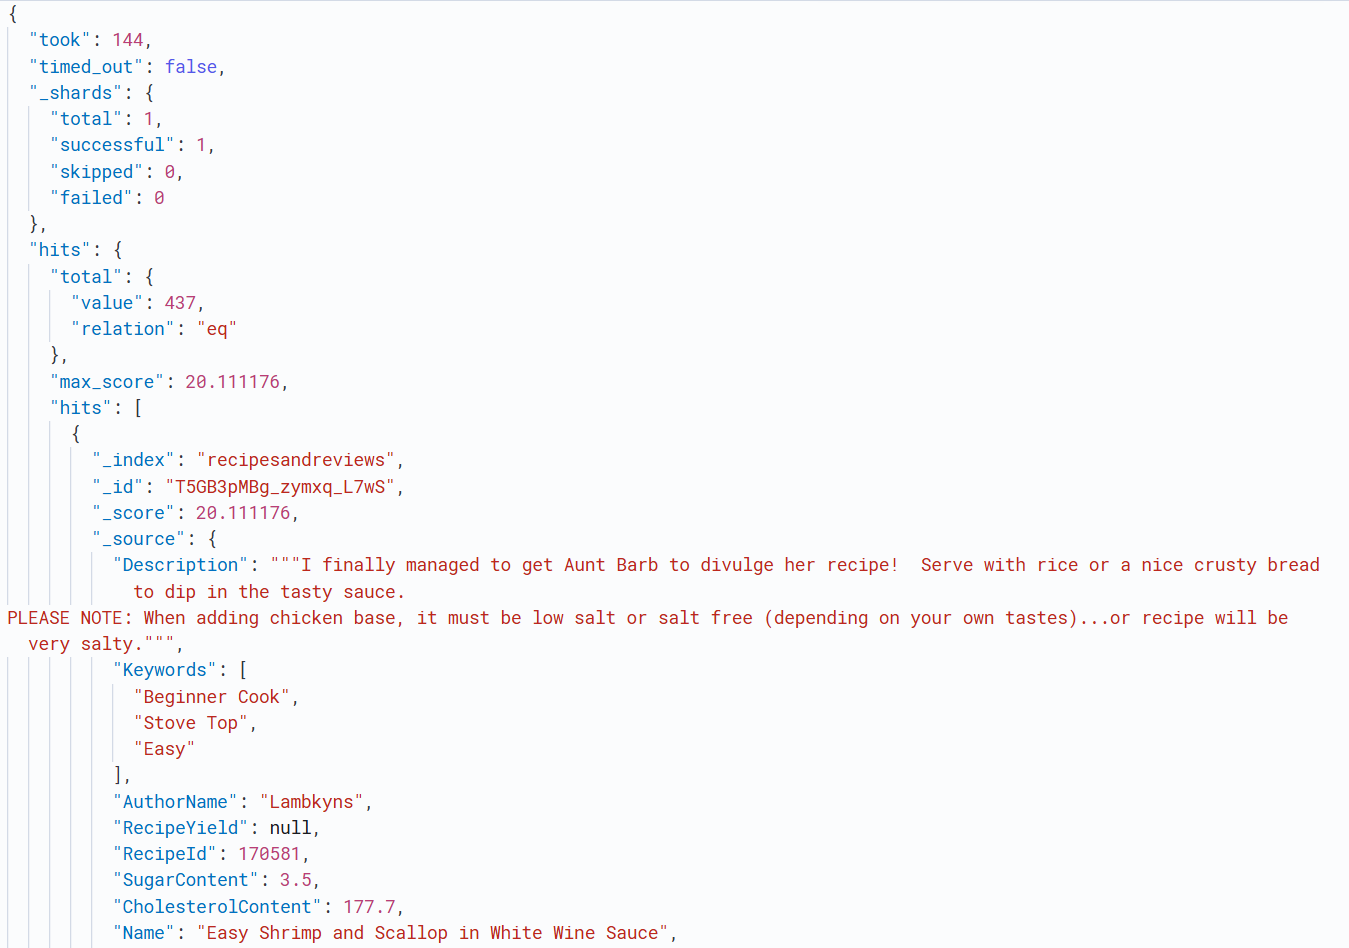
\includegraphics[width=0.8\linewidth]{Report/ReportLatex/Images/ElasticsearchResults/RomanticDinner1.png}
    \caption{1st result}
    \label{fig:enter-label}
    \end{figure}
    \begin{figure}[H]
    \centering
    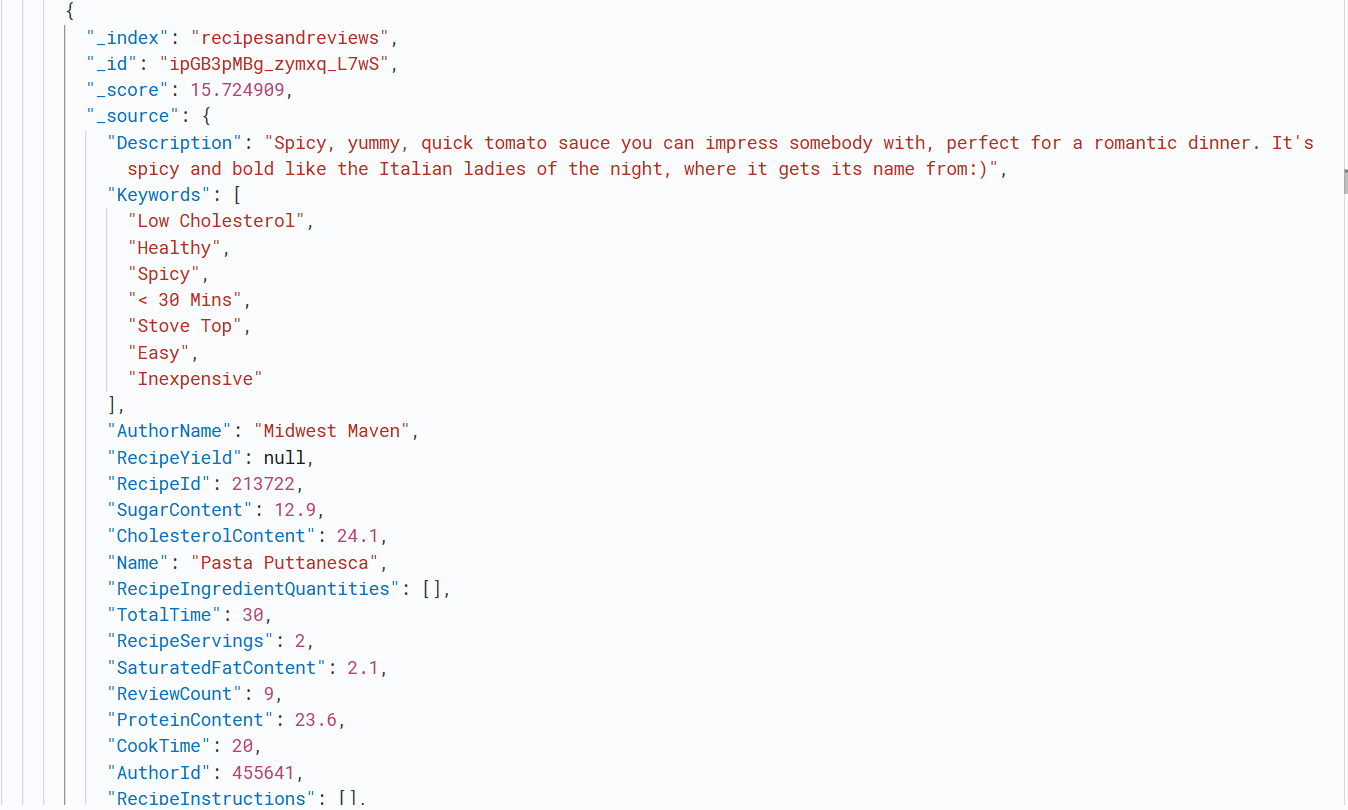
\includegraphics[width=0.9\linewidth]{Report/ReportLatex/Images/ElasticsearchResults/RomanticDinner2.png}
    \caption{2nd result}
    \label{fig:enter-label}
    \end{figure}
    \clearpage
    
    \item \textbf{Recipes made only using a microwave }

    This query is designed to help a student who only has a microwave and no other appliances find recipes that can be made exclusively with a microwave.
    
    In the must clause, we ensure that the RecipeInstructions field contains the word "microwave", confirming that the recipe involves using the microwave for cooking. To further refine the search, we added a must\_not clause to exclude any recipes that mention the use of other appliances, such as an oven, pan, pot, or fryer, in the Keywords or RecipeInstructions fields. This ensures that only recipes that rely solely on the microwave are included in the results.

    Additionally, the should clause is used to give a higher score to recipes that highlight the microwave as a key element. We search for the term "microwave" in the Keywords and in the Reviews.Review field, as they indicate that the microwave is an important part of the recipe according to either the recipe creator or reviewers.

    This approach ensures that the student will find recipes that are specifically designed for a microwave, without needing any additional cooking appliances, and gives extra weight to those that emphasize the microwave's role in the cooking process. We chose to not put a minimum should match since here the only foundamental parameters are those in the must and must not clause.

    \subsubsection{Query}
    \begin{verbatim}
GET /recipesandreviews/_search
{
  "query": {
    "bool": {
      "must": [
        {
          "match": {
            "RecipeInstructions": "microwave"
          }}],
      "must_not": [
        {
          "match": {
            "Keywords": {
              "query": "oven pan pot fryer",
              "operator": "or"
            }}},
        {
          "match": {
            "RecipeInstructions": {
              "query": "oven pan pot fryer",
              "operator": "or"
            }}}],
      "should": [
        {
          "match": {
            "Keywords": "microwave"
          }},
        {
          "nested": {
            "path": "Reviews",
            "query": {
              "match": {
                "Reviews.Review": "microwave"
              }}}}]}}}
    \end{verbatim}

    \subsubsection{Result}
    Here we show the beginning of the first 2 output documents given by the query. 
    \begin{figure}[H]
    \centering
    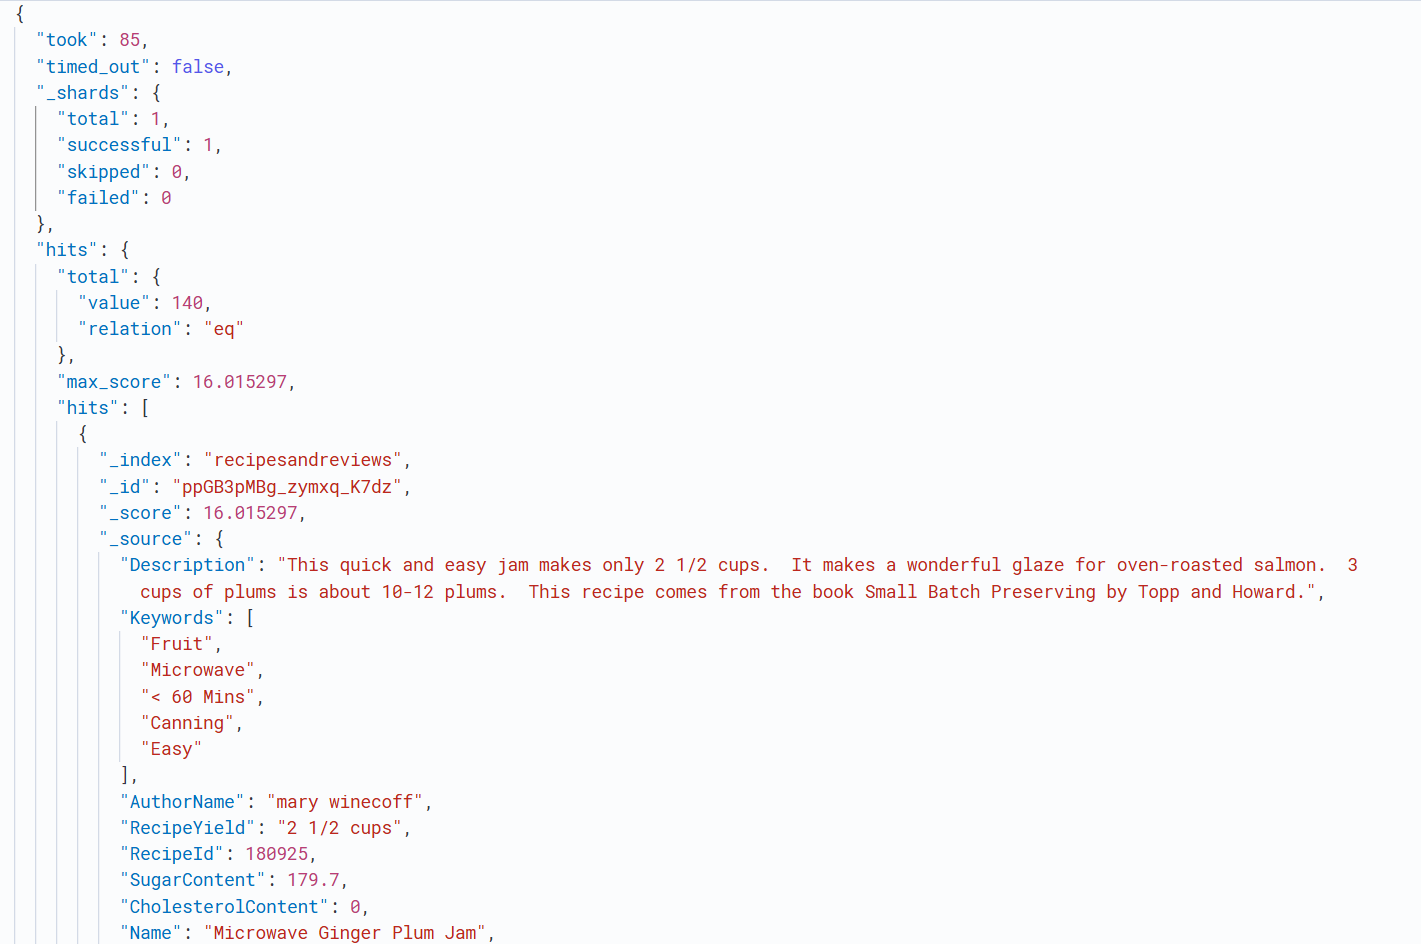
\includegraphics[width=0.8\linewidth]{Report/ReportLatex/Images/ElasticsearchResults/microwave1.png}
    \caption{1st result}
    \label{fig:enter-label}
    \end{figure}
    \begin{figure}[H]
    \centering
    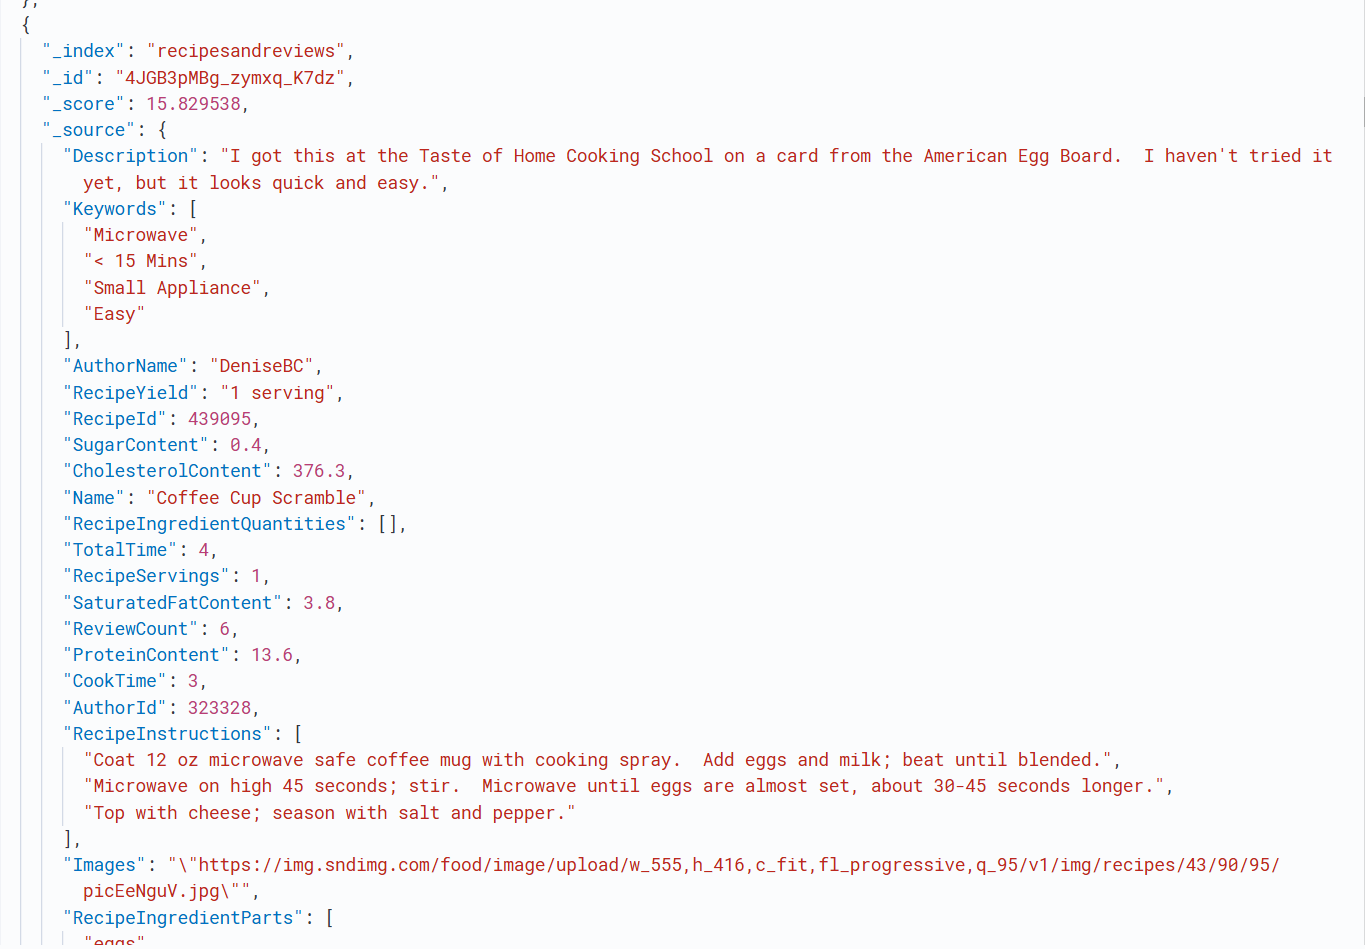
\includegraphics[width=0.9\linewidth]{Report/ReportLatex/Images/ElasticsearchResults/microwave2.png}
    \caption{2nd result}
    \label{fig:enter-label}
    \end{figure}
    \clearpage
    
    \item \textbf{Quick Recipes Using All Given Ingredients}

    This query was designed to find recipes that use all the ingredients provided by a user. To achieve this, we employed a must clause that contains a match query and a range query. 
    
    The match query searches for the specified ingredients within the RecipeIngredientParts field (a text field). To ensure all ingredients are included, the match query uses an and operator, meaning only recipes that contain all the listed ingredients will be returned.
    
    The range query filters recipes to include only those with a total time of 30 minutes or less, fulfilling the requirement for quick recipes.
    \subsubsection{Query}
    \begin{verbatim}
GET /recipesandreviews/_search
{
  "query": {
    "bool": {
      "must": [
        {
          "match": {
            "RecipeIngredientParts": {
              "query": "chicken onion cheese",
              "operator": "and"
            }}},
        {
          "range": {
            "TotalTime": {
              "lte": 30
            }}}]}}}
    \end{verbatim}

    \subsubsection{Result}
    Here, we present the beginning of the output, including the metadata and several images displaying the RecipeIngredientParts field from various recipes, to show the accuracy of the results.
    \begin{figure}[H]
    \centering
    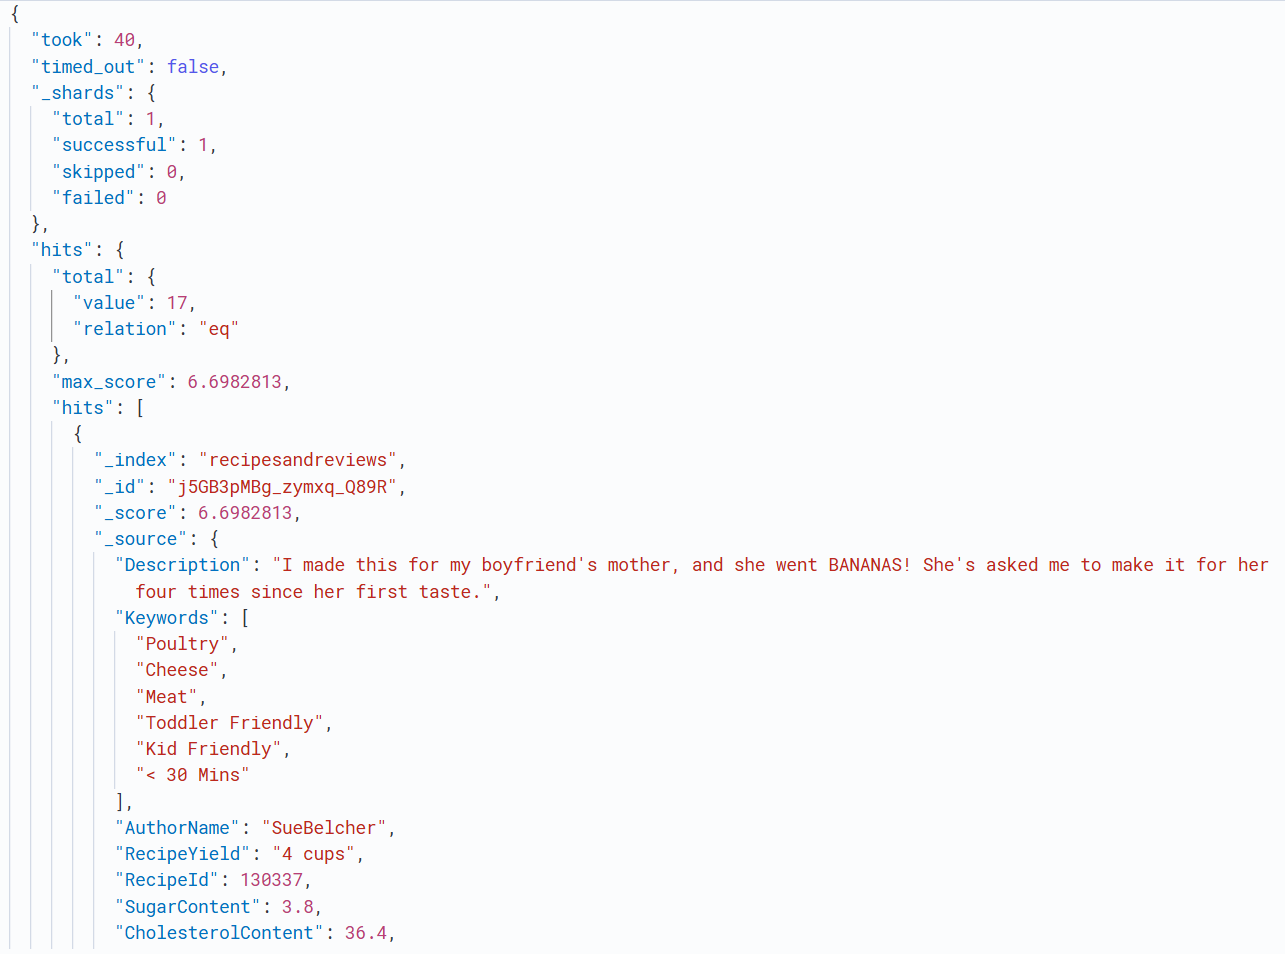
\includegraphics[width=0.9\linewidth]{Report/ReportLatex/Images/ElasticsearchResults/ingredients1.png}
    \caption{1st result}
    \label{fig:enter-label}
    \end{figure}

    \begin{figure}[h!]
    \centering
    \begin{minipage}{0.25\textwidth}
        \centering
        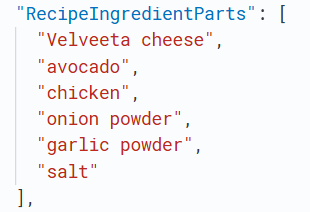
\includegraphics[width=\textwidth]{Report/ReportLatex/Images/ElasticsearchResults/ingredients2.png}
    \end{minipage}%
    \hspace{0.05\textwidth}
    \begin{minipage}{0.25\textwidth}
        \centering
        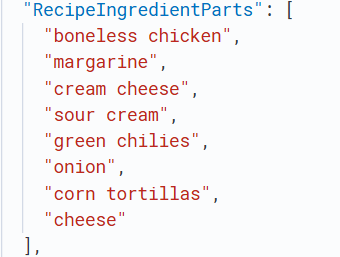
\includegraphics[width=\textwidth]{Report/ReportLatex/Images/ElasticsearchResults/ingredients3.png}
    \end{minipage}%
    \hspace{0.05\textwidth}
    \begin{minipage}{0.25\textwidth}
        \centering
        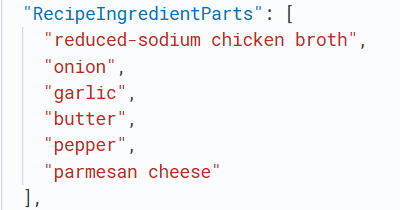
\includegraphics[width=\textwidth]{Report/ReportLatex/Images/ElasticsearchResults/ingredients4.png}
    \end{minipage}
    
    \caption{RecipeIngredientParts}
    \end{figure}
    \clearpage
    
    \item \textbf{Recipes for a party with a lot of servings}
    
    To find recipes suitable for hosting a party, we focused on identifying those that serve a larger number of people. In the must clause, we specified that the recipes should have a RecipeServings greater than or equal to 10, ensuring that they are fit for a gathering. Additionally, we applied a should clause to give extra weight to recipes that explicitly reference terms associated with parties and large events, such as "party," "large groups," "gathering," "celebration," "buffet," and similar phrases.

    The should clause includes several fields where these keywords might appear, for example, the Keywords field is searched for terms like "party" and "celebration," with a boost of 2, emphasizing recipes designed with these themes in mind. The RecipeCategory field is also considered, with a boost of 1.5 for categories such as "Party," "Buffet," and "Appetizer," since these are often associated with party-friendly meals. Similarly, the Description field is searched for party-related terms with a boost of 1.5 to highlight recipes that mention large gatherings or events.
    Lastly, we included the Reviews field, specifically searching within the nested Reviews.Review subfield for mentions of party-related terms. These reviews are boosted with a higher weight (boost of 3)  since we thought that in this context the reviews are the most important parameter to account for.
    The minimum\_should\_match parameter is set to 1, ensuring that at least one of the should conditions is be satisfied for a recipe to be returned in the results

    \subsubsection{Query}
    \begin{verbatim}
GET /recipesandreviews/_search
{
  "query": {
    "bool": {
      "must": [
        {
          "range": {
            "RecipeServings": {
              "gte": 10
            }}}],
      "should": [
        {
          "match": {
            "Keywords": {
              "query": "party, large groups, gathering, celebration, 
              event, buffet",
              "operator": "or",
              "boost": 2
            }}},
        {
          "match": {
            "RecipeCategory": {
              "query": "Dessert, Appetizer, Main, Party, Buffet",
              "operator": "or",
              "boost": 1.5
            }}},
        {
          "match": {
            "Description": {
              "query": "party, large groups, gathering, celebration, event",
              "operator": "or",
              "boost": 1.5
            }}},
        {
          "nested": {
            "path": "Reviews",
            "query": {
              "match": {
                "Reviews.Review": {
                  "query": "party, celebration, gathering, event, buffet",
                  "operator": "or",
                  "boost": 3
                }}}}}],
      "minimum_should_match": 1
    }}}
    \end{verbatim}

    \subsubsection{Result}
    In the first image, we display the first result along with the prior metadata. In the second image, we highlight some of the reviews in the output, demonstrating that the query successfully retrieved relevant recipes.
    \begin{figure}[H]
    \centering
    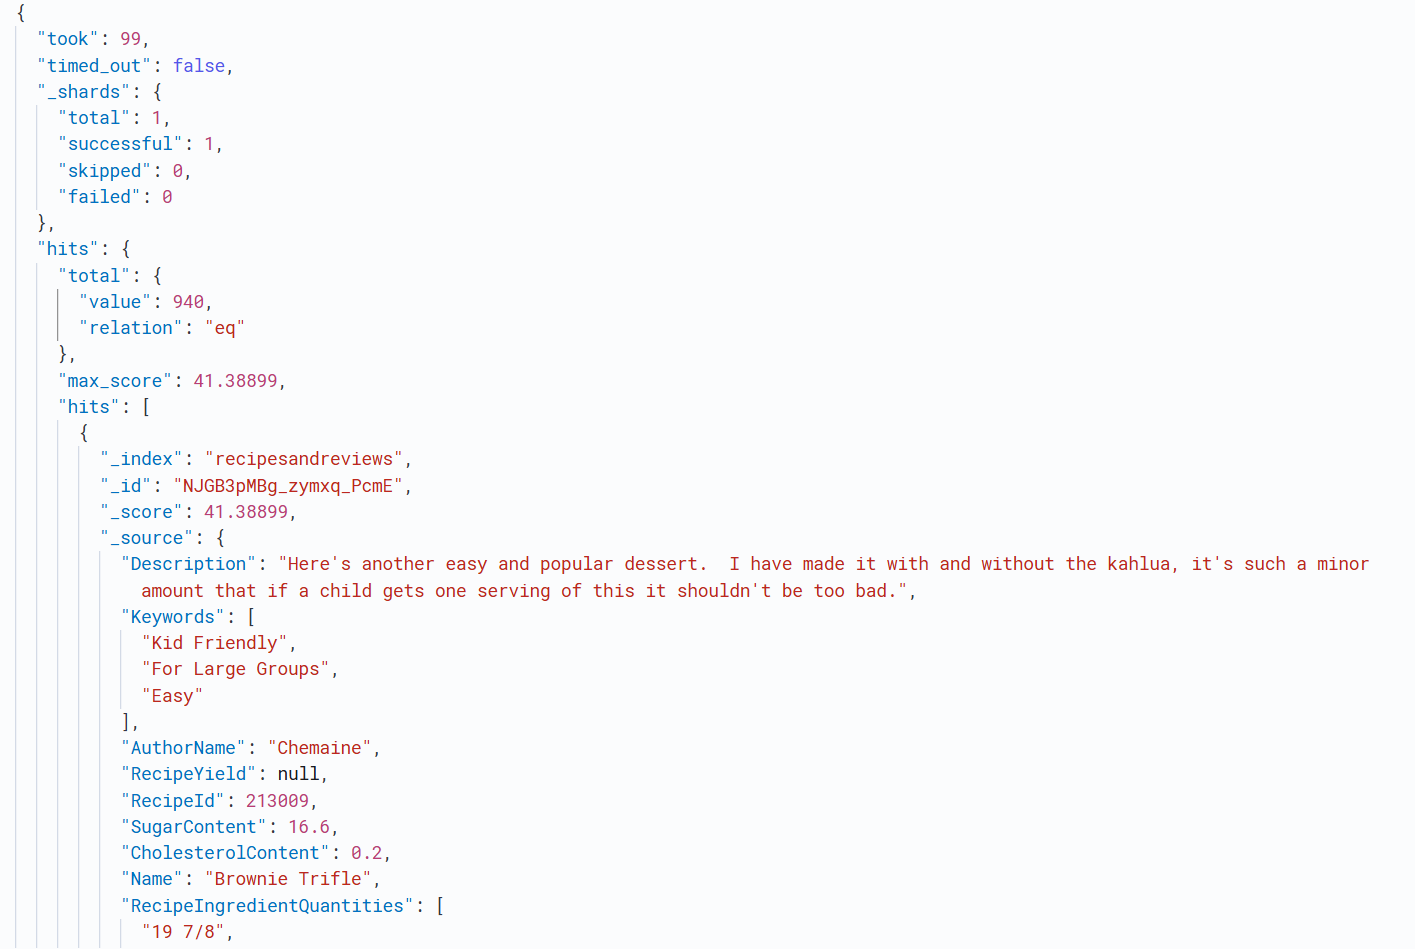
\includegraphics[width=0.9\linewidth]{Report/ReportLatex/Images/ElasticsearchResults/party1.png}
    \caption{1st result}
    \label{fig:enter-label}
    \end{figure}
    \begin{figure}[H]
    \centering
    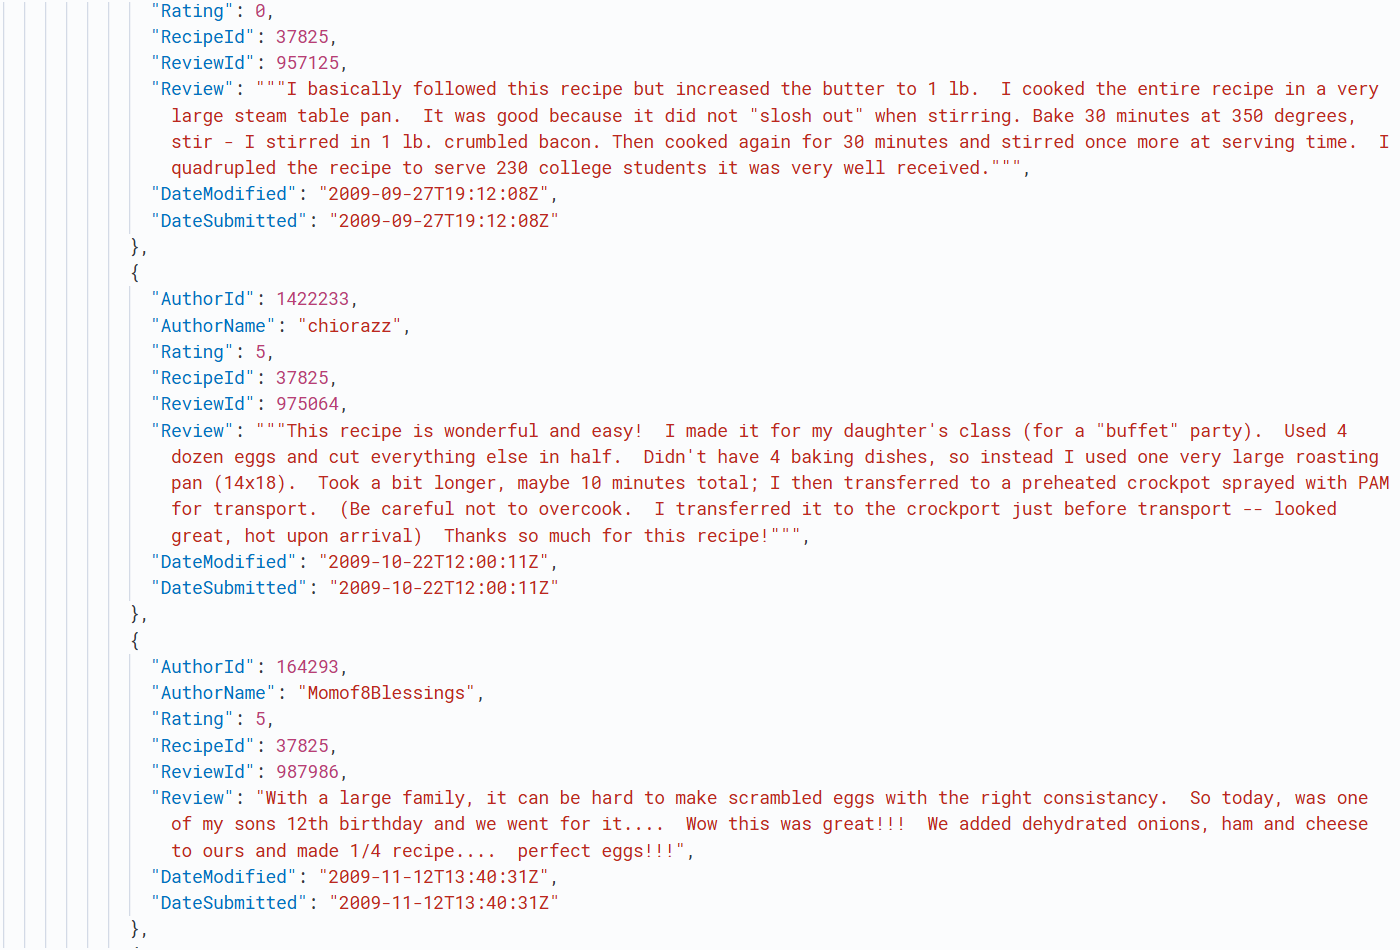
\includegraphics[width=0.9\linewidth]{Report/ReportLatex/Images/ElasticsearchResults/party2.png}
    \caption{Relevant Reviews}
    \label{fig:enter-label}
    \end{figure}
    \clearpage
    
    \item \textbf{Recipes with the best protein/calorie ratio}

    This Elasticsearch query identifies recipes that are high in protein relative to their calorie content and associated with keywords related to health, fitness, and nutrition. It combines a script-based filter with a relevance scoring system to prioritize results that align with the criteria in the should clause.

    The script filters recipes by calculating the protein to/calorie ratio dynamically. It includes recipes where calories are non-zero, and protein makes up at least 20\% of the total calories. This approach avoids the need to precompute and store the ratio as a separate field, offering flexibility to adapt the logic without re-indexing. 

    The query also ranks recipes higher if they match specific health-related keywords in their description, keywords, recipe category, or user reviews. We use words like "healthy," "gym," "protein," "fit," and "nutritious" to search for this concept in the data.

    \begin{verbatim}
GET /recipesandreviews/_search
{
  "query": {
    "bool": {
      "filter": [
        {
          "script": {
            "script": {
              "source": """
                if (doc['Calories'].size() > 0 && doc['Calories'].value != 0) {
                  return doc['ProteinContent'].value / doc['Calories'].value >= 0.2;
                } else {
                  return false;
                }
              """
            }}}],
      "should": [
        {
          "match": {
            "Description": {
              "query": "healthy gym protein fit strong weight nutritious",
              "operator": "or"
              }}},
        {
          "match": {
            "Keywords": {
              "query": "healthy gym protein fit strong weight nutritious",
              "operator": "or",
              "boost": 3
              }}},
        {
          "match": {
            "RecipeCategory": {
              "query": "healthy gym protein fit strong weight nutritious",
              "operator": "or"
              }}},
        {
          "nested": {
            "path": "Reviews",
              "query": {
                "match": {
                  "Reviews.Review": {
                    "query": "healthy gym protein fit strong weight nutritious",
                    "operator": "or"
                    }}}}}]}}}
    \end{verbatim}

    \subsubsection{Result}
    Here we show the beginning of the first 2 output documents given by the query. 
    \begin{figure}[H]
    \centering
    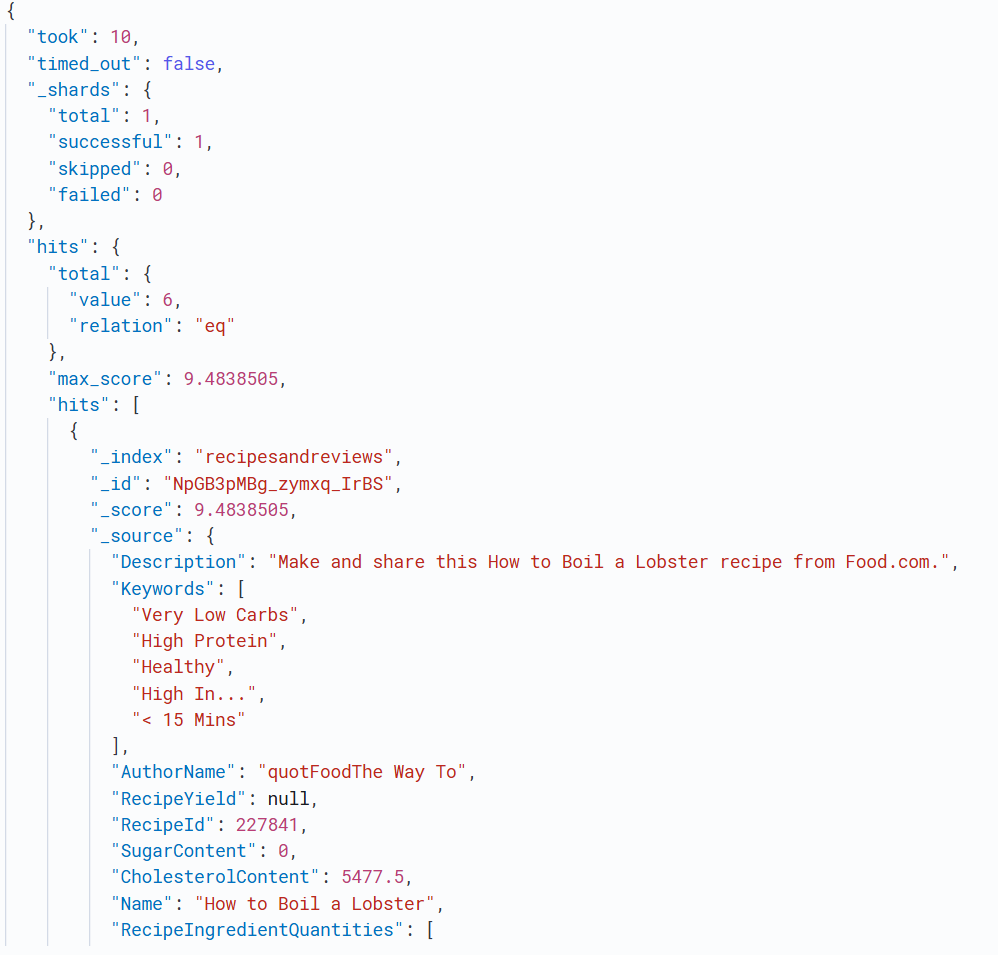
\includegraphics[width=0.8\linewidth]{Report/ReportLatex/Images/ElasticsearchResults/proteins1.png}
    \caption{1st result}
    \label{fig:enter-label}
    \end{figure}
    \begin{figure}[H]
    \centering
    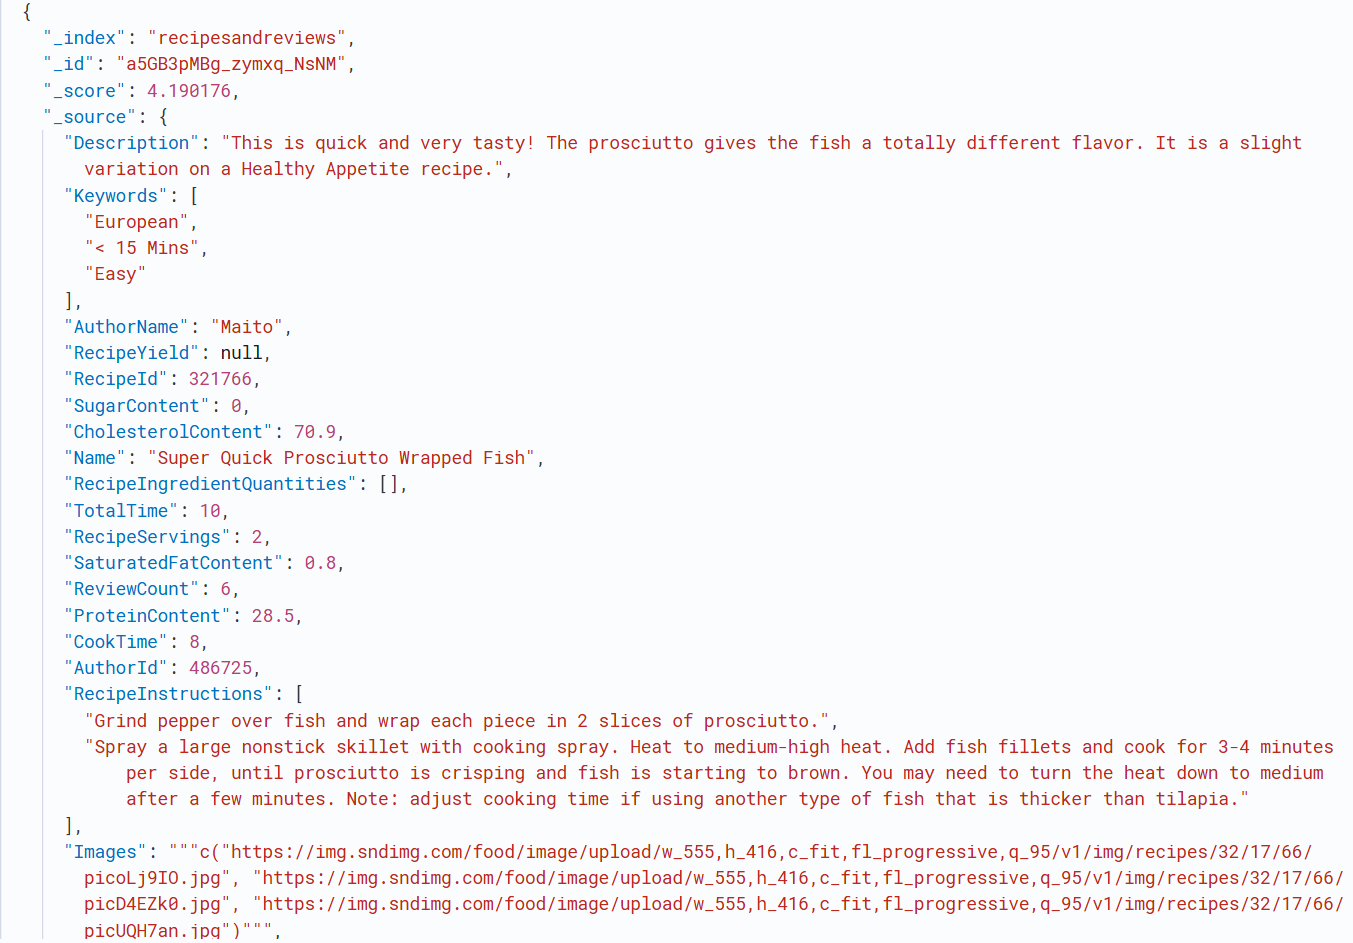
\includegraphics[width=0.8\linewidth]{Report/ReportLatex/Images/ElasticsearchResults/proteins2.png}
    \caption{2nd result}
    \label{fig:enter-label}
    \end{figure}
    
    \clearpage
    
    \item \textbf{Recipes for specific dietary restrictions (lactose intolerance)}

    This query is designed to find recipes suitable for individuals with lactose intolerance or those following a lactose-free diet. The search first excludes any recipes containing common sources of lactose, such as milk, cheese, lactose, and yogurt, using the must\_not clause. This ensures that recipes with these ingredients are filtered out, as they are not appropriate for people who need to avoid lactose.

    In addition to filtering out lactose-containing ingredients, the query uses a should clause to boost the relevance of recipes that explicitly mention being lactose-free or suitable for those with lactose intolerance. It looks for these terms in the Keywords, Description, and RecipeCategory fields, as well as in Reviews. The query searches for terms like "lactose free" and "lactose intolerant" across these fields to give higher scores to recipes that are clearly labeled as suitable for those with lactose restrictions. This helps prioritize lactose-free recipes, making it easier for users to find meals that meet their dietary needs.

    \begin{verbatim}
GET /recipesandreviews/_search
{
  "query": {
    "bool": {
      "must_not": [
        {
          "match": {
            "RecipeIngredientParts": {
              "query": "milk cheese lactose yogurt",
              "operator": "or"
            }}}],
      "should": [
        {
          "match": {
            "Keywords": "lactose free"
          }},
        {
          "match": {
            "Description": "lactose free intolerant"
          }},
        {
          "match": {
            "RecipeCategory": "lactose free"
          }},
        {
          "nested": {
            "path": "Reviews",
            "query": {
              "match": {
                "Reviews.Review": "lactose free intolerant"
              }}}}]}}}
    \end{verbatim}

    \subsubsection{Result}
    In the images, we display the beginning of the first and the second result along with the prior metadata.
    \begin{figure}[H]
    \centering
    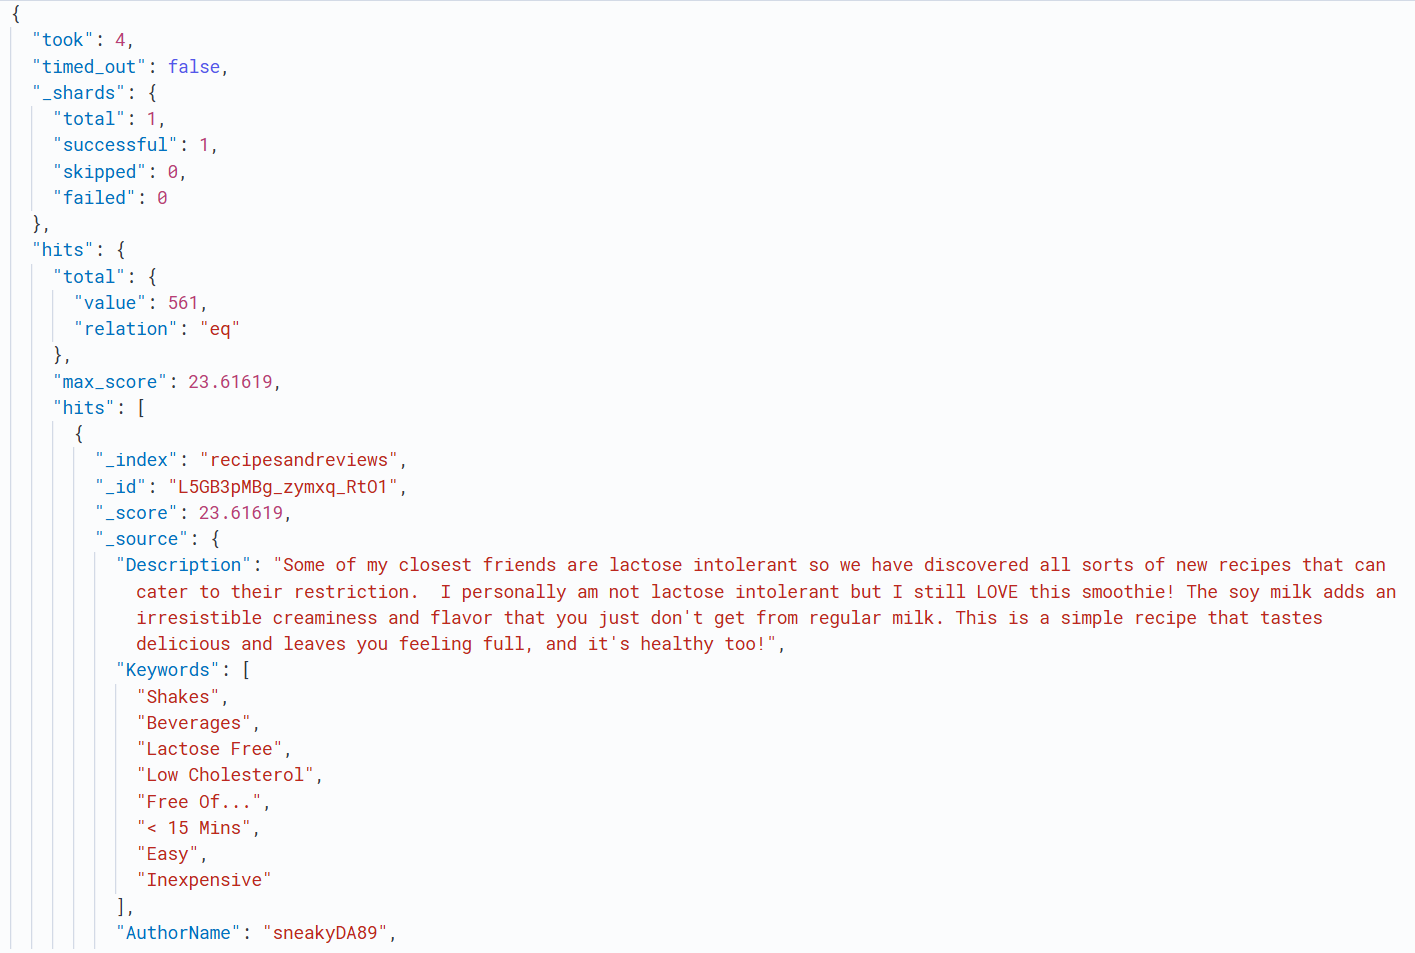
\includegraphics[width=0.9\linewidth]{Report/ReportLatex/Images/ElasticsearchResults/lactose1.png}
    \caption{1st result}
    \label{fig:enter-label}
    \end{figure}
    \begin{figure}[H]
    \centering
    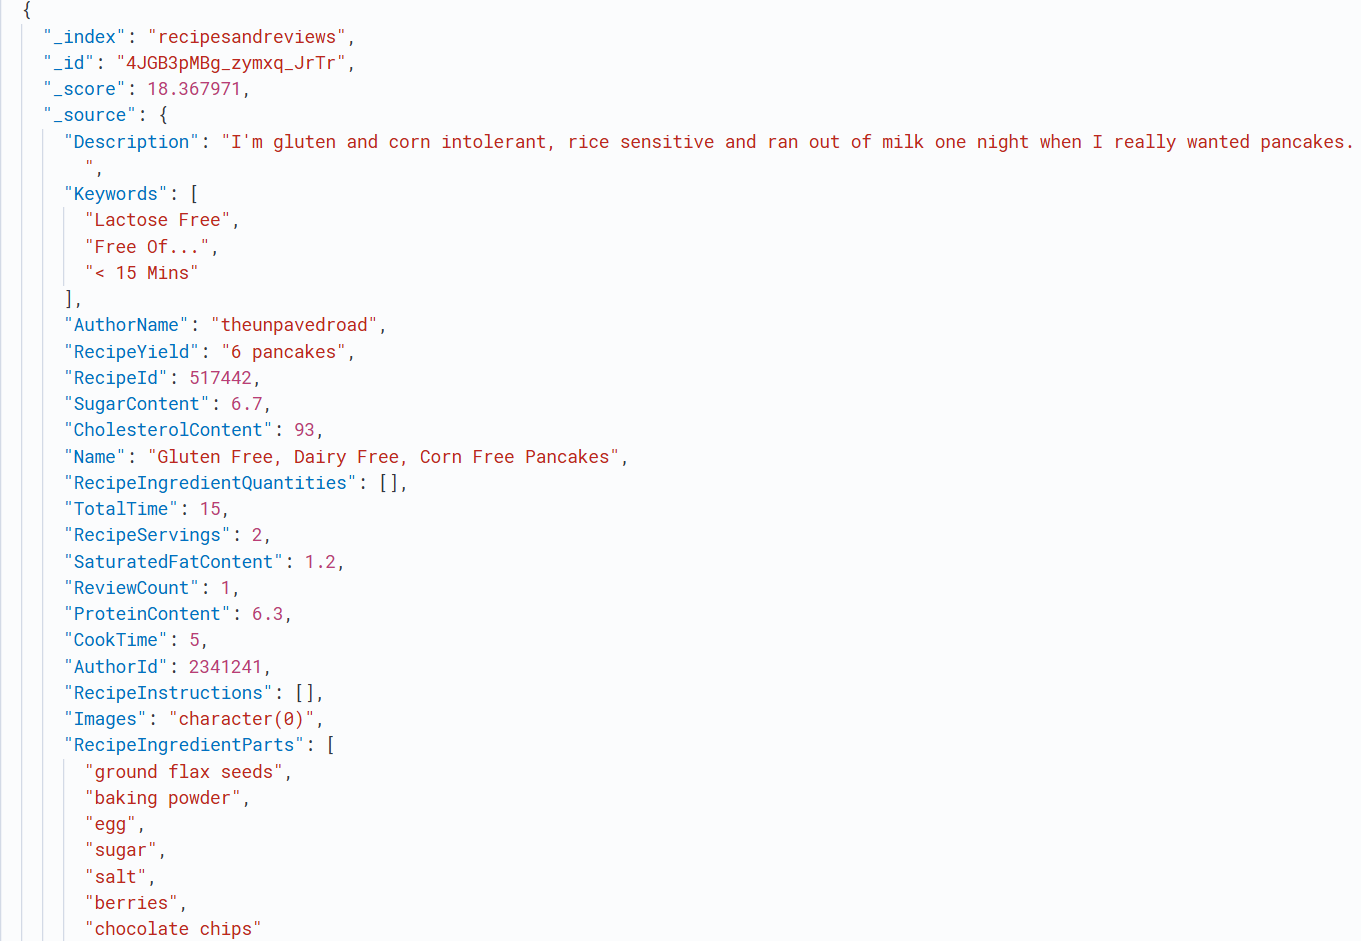
\includegraphics[width=0.9\linewidth]{Report/ReportLatex/Images/ElasticsearchResults/lactose2.png}
    \caption{2nd result}
    \label{fig:enter-label}
    \end{figure}
    \clearpage
    
    \item \textbf{Query to analyze the correlation between macronutrient ranges and calorie content}

    This Elasticsearch query is designed to analyze the relationship between calorie content and macronutrient distribution in recipes, aiming to uncover potential correlations. Recipes are grouped into predefined calorie ranges—low (under 1400 calories), medium (1400 to 2000 calories), and high (over 2000 calories). Within each calorie range, recipes are further categorized based on their levels of protein, fat, fiber, and sugar. Each nutrient is divided into three ranges: low, medium, and high, defined by thresholds such as grams of protein, fat, fiber, or sugar.

    The query uses a top-level aggregation to group recipes by calorie ranges. Nested within each calorie group, sub-aggregations further divide recipes into nutrient-specific ranges, such as low protein (less than 5g), medium fat (5–15g), or high sugar (more than 15g). The focus is not on retrieving individual recipes but on generating summarized data that describes the nutritional characteristics within each calorie group.

    This approach allows for the examination of how macronutrient levels vary with calorie content, helping to identify trends or patterns. The results from this query were then used to create a heatmap, visually highlighting the relationships and correlations between calorie ranges and macronutrient levels, that we will show in the following chapter about Extras.
    
    \begin{verbatim}
GET /recipesandreviews/_search
{
  "size": 0,
  "aggs": {
    "calorie_ranges": {
      "range": {
        "field": "Calories",
        "ranges": [
          { "to": 1400, "key": "Low calorie" },
          { "from": 1400, "to": 2000, "key": "Medium calorie" },
          { "from": 2000, "key": "High calorie" }
        ]},
      "aggs": {
        "protein_ranges": {
          "range": {
            "field": "ProteinContent",
            "ranges": [
              { "to": 5, "key": "Low protein" },
              { "from": 5, "to": 15, "key": "Medium protein" },
              { "from": 15, "key": "High protein" }
            ]}},
        "fat_ranges": {
          "range": {
            "field": "FatContent",
            "ranges": [
              { "to": 5, "key": "Low fat" },
              { "from": 5, "to": 15, "key": "Medium fat" },
              { "from": 15, "key": "High fat" }
            ]}},
        "fiber_ranges": {
          "range": {
            "field": "FiberContent",
            "ranges": [
              { "to": 1, "key": "Low fiber" },
              { "from": 1, "to": 5, "key": "Medium fiber" },
              { "from": 5, "key": "High fiber" }
            ]}},
        "sugar_ranges": {
          "range": {
            "field": "SugarContent",
            "ranges": [
              { "to": 5, "key": "Low sugar" },
              { "from": 5, "to": 15, "key": "Medium sugar" },
              { "from": 15, "key": "High sugar" }
            ]}}}}}}
    \end{verbatim}

    \subsubsection{Result}
    In the images, we display the ouput up to the end of the first bucket aggregation (low calorie)

    \begin{figure}[h!]
    \centering
    \begin{minipage}{0.25\textwidth}
        \centering
        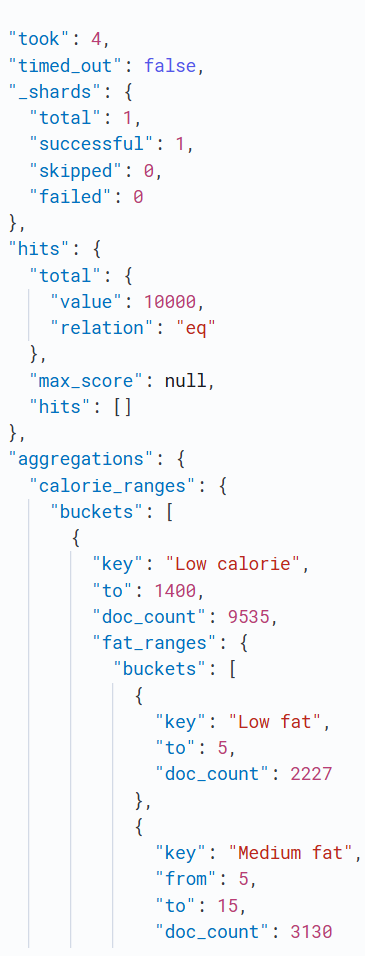
\includegraphics[width=\textwidth]{Report/ReportLatex/Images/ElasticsearchResults/calories1.png}
    \end{minipage}%
    \hspace{0.05\textwidth}
    \begin{minipage}{0.25\textwidth}
        \centering
        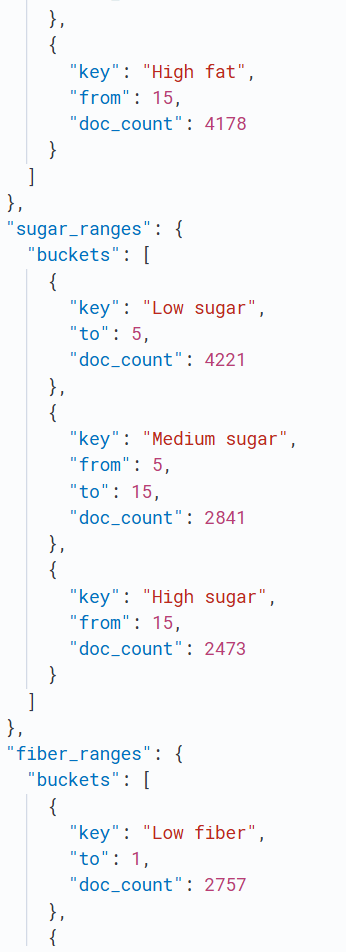
\includegraphics[width=\textwidth]{Report/ReportLatex/Images/ElasticsearchResults/calories2.png}
    \end{minipage}%
    \hspace{0.05\textwidth}
    \begin{minipage}{0.25\textwidth}
        \centering
        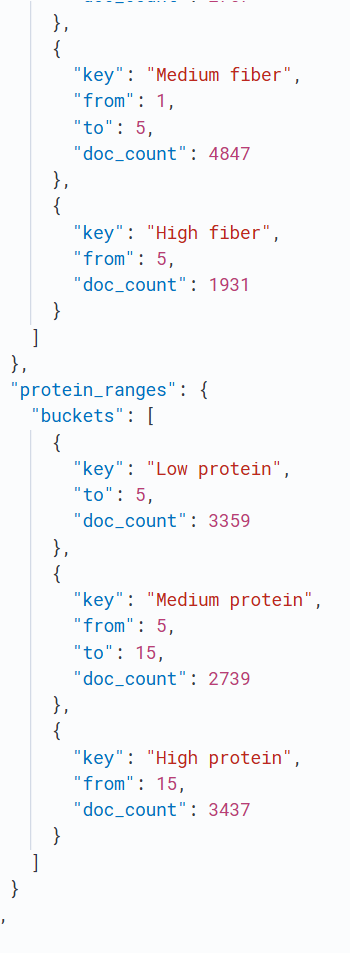
\includegraphics[width=\textwidth]{Report/ReportLatex/Images/ElasticsearchResults/calories3.png}
    \end{minipage}
    
    \caption{Output}
    \end{figure}
    
    \clearpage
    
    \item \textbf{Healthy, high-protein snacks that are not desserts}

    This query is designed to find snack recipes that are specifically healthy and high in protein, while excluding any recipes that fall under the dessert category. It starts by using the must clause to filter recipes that fall into the "Snacks" category and contain at least 20 grams of protein. These two conditions ensure that the results are relevant to the searcher's criteria for protein-packed snacks.

    In addition to these foundational requirements, the query includes a should clause to boost recipes that explicitly reference "healthy snack" in the description, reviews, or keywords. The use of the operator: "and" within the match queries means that the terms "healthy" and "snack" must both be present in these fields, increasing the likelihood of finding recipes that are truly aligned with the searcher's goal of a healthy, protein-rich snack.

    Furthermore, the query includes a must\_not clause to explicitly exclude recipes that are categorized as "dessert" or contain the term "dessert" in their keywords. This is important because the user wants to avoid any recipes that may be high in sugar or calories, which are often found in dessert items.

    \begin{verbatim}
GET /recipesandreviews/_search
{
  "query": {
    "bool": {
      "must":[
        {"match": {"RecipeCategory": "Snacks"}},
        {"range": { "ProteinContent": { "gte": 20 } } }
      ],
      "should": [
        { "match": { 
            "Description": {
              "query": "healthy snack",
              "operator": "and"
            } } },
        {
          "nested": {
            "path": "Reviews",
            "query": {
              "match": {
                "Reviews.Review": {
                  "query": "healthy snack",
                  "operator": "and"
                }}}}},
        {
          "match": {
            "Keywords": {
              "query": "healthy snack"
            }}}],
      "must_not": [
        { "match":{"RecipeCategory": "dessert"} },
        { "match":{"Keywords": "dessert"} }
      ]}}}
    \end{verbatim}

    \subsubsection{Result}
    In the images, we display the beginning of the first and the second result along with the prior metadata.
    \begin{figure}[H]
    \centering
    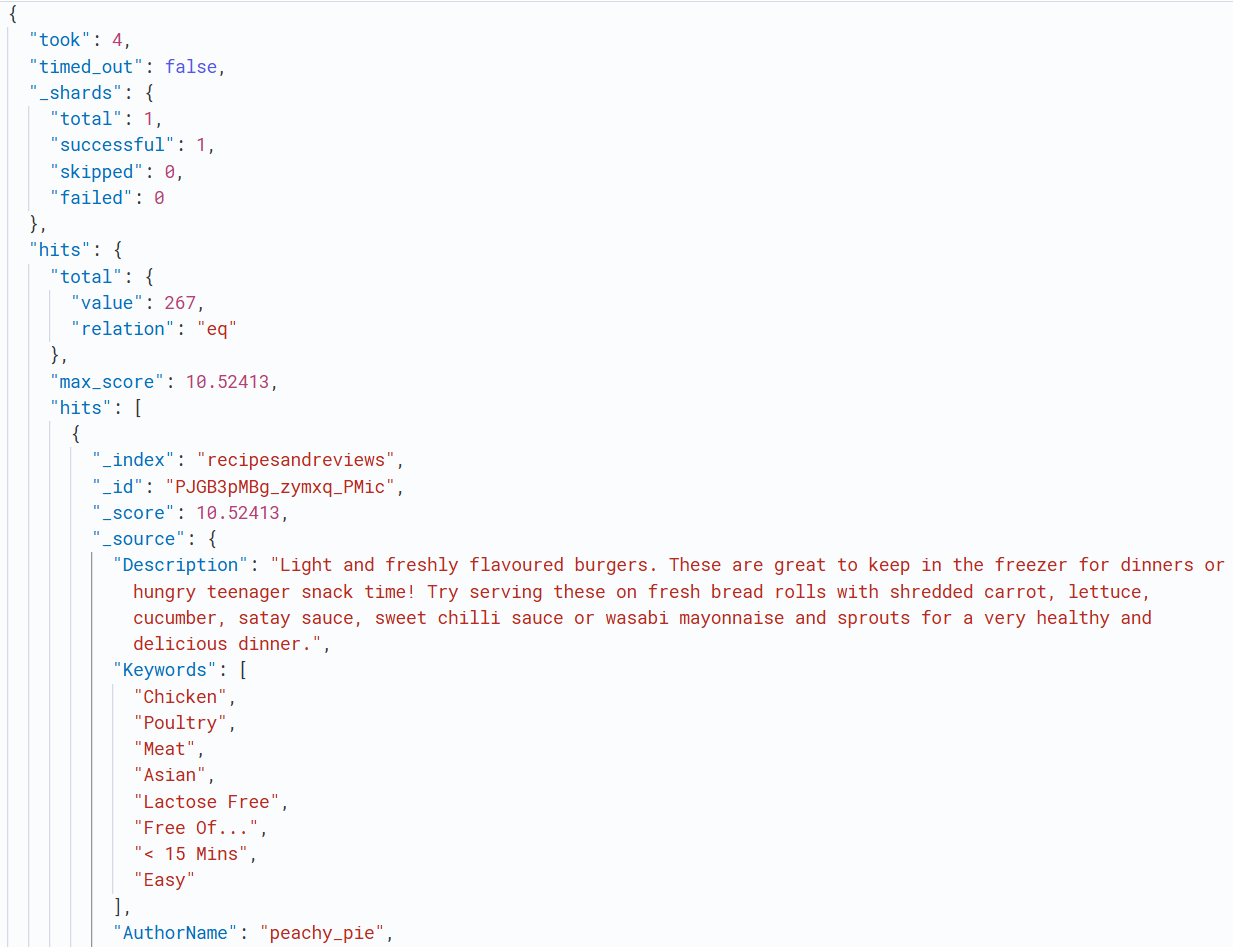
\includegraphics[width=0.8\linewidth]{Report/ReportLatex/Images/ElasticsearchResults/snack1.png}
    \caption{1st result}
    \label{fig:enter-label}
    \end{figure}
    \begin{figure}[H]
    \centering
    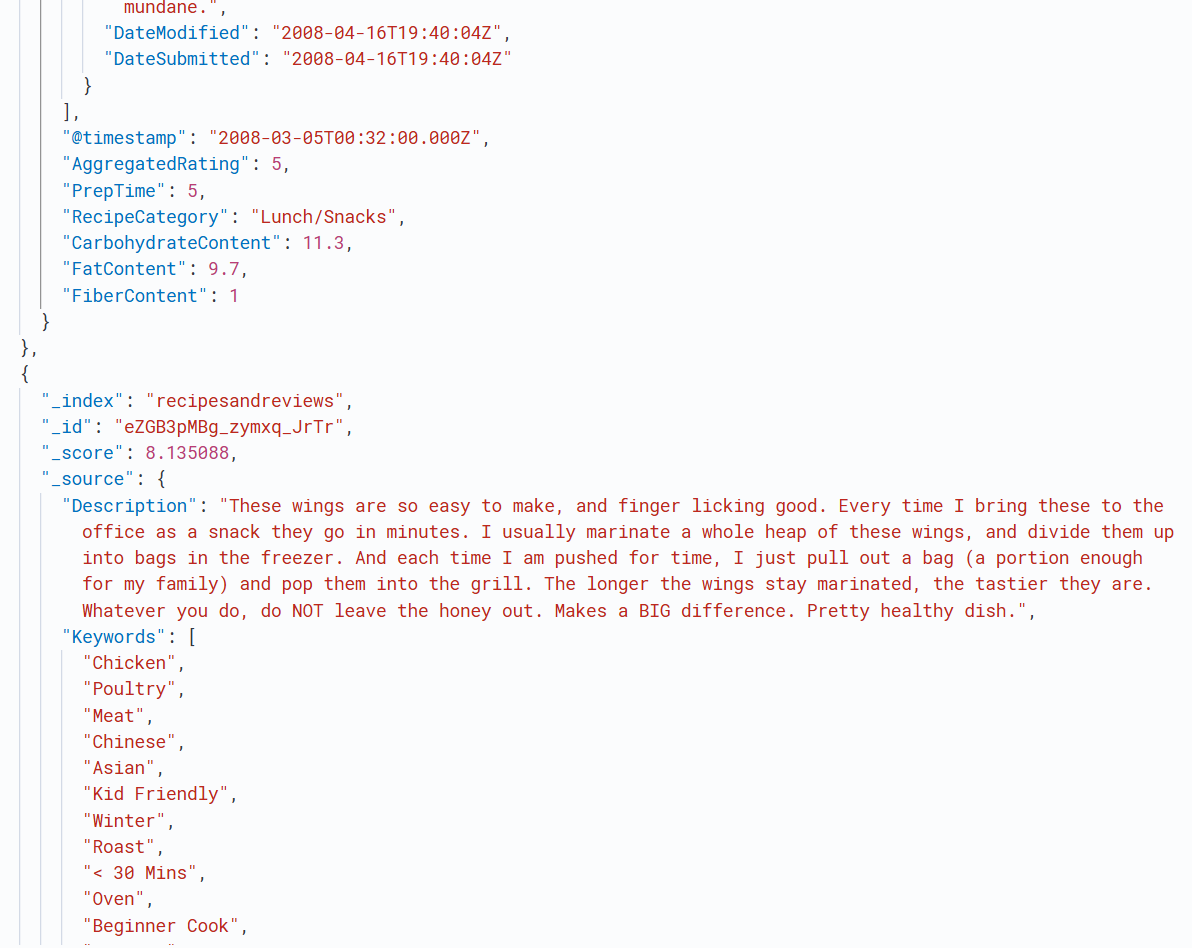
\includegraphics[width=0.8\linewidth]{Report/ReportLatex/Images/ElasticsearchResults/snack2.png}
    \caption{2nd result}
    \label{fig:enter-label}
    \end{figure}
    \clearpage
    
    \clearpage
    
    \item \textbf{Query that finds the authors with the best reviews}

    This query is designed for users who are looking to find accredited recipe authors to be inspired by, based on the quality of their recipes and the positive feedback they receive. By identifying authors with the best-reviewed recipes, this query helps users discover trustworthy sources for highly-rated dishes.

    The search starts with a must clause to ensure that only recipes with an AggregatedRating of 4 or higher are included, meaning the recipes are highly rated. Additionally, it filters out recipes with fewer than 10 reviews using a range query within the must clause on the ReviewCount field. This ensures that the results represent recipes that are well-reviewed by a significant number of people, giving a more reliable picture of the author's reputation.

    To further refine the results, the query includes a nested query within the Reviews field, looking for specific positive terms such as "great," "excellent," "good," "amazing," and "awesome." This helps identify recipes that have reviews with a positive sentiment. The operator: "or" in the query ensures that any of these positive words will contribute to the match, making it easier to capture a variety of positive sentiments across different reviews.

    The aggregation part of the query then groups the results by AuthorId using a terms aggregation, which enables the query to list authors who have the best reviews. Within each author group, the average\_rating aggregation computes the average AggregatedRating for their recipes. This provides a way to rank authors based on the quality of their work, specifically those who consistently receive high ratings.

    \begin{verbatim}
GET /recipesandreviews/_search
{
  "size": 1,
  "query": {
    "bool": {
      "must": [
        {"range": { "AggregatedRating": { "gte": 4} } },
        {"range": { "ReviewCount": { "gte": 10 } } },
        {"nested":{
          "path": "Reviews",
          "query": {
            "match": {
              "Reviews.Review": {
                "query": "great excellent good amazing awesome delicious yummy",
                "operator": "or"
            }}}}}]}},
  "aggs": {
    "positive_sentiment_per_author": {
      "terms": {
        "field": "AuthorId"
      },
      "aggs": {
        "average_rating": {
          "avg": {
            "field": "AggregatedRating"
          }}}}}}
    \end{verbatim}

    \subsubsection{Result}
    In the pictures below we display the first document returned by the query and the beginning of the output section displaying aggregations.
    \begin{figure}[H]
    \centering
    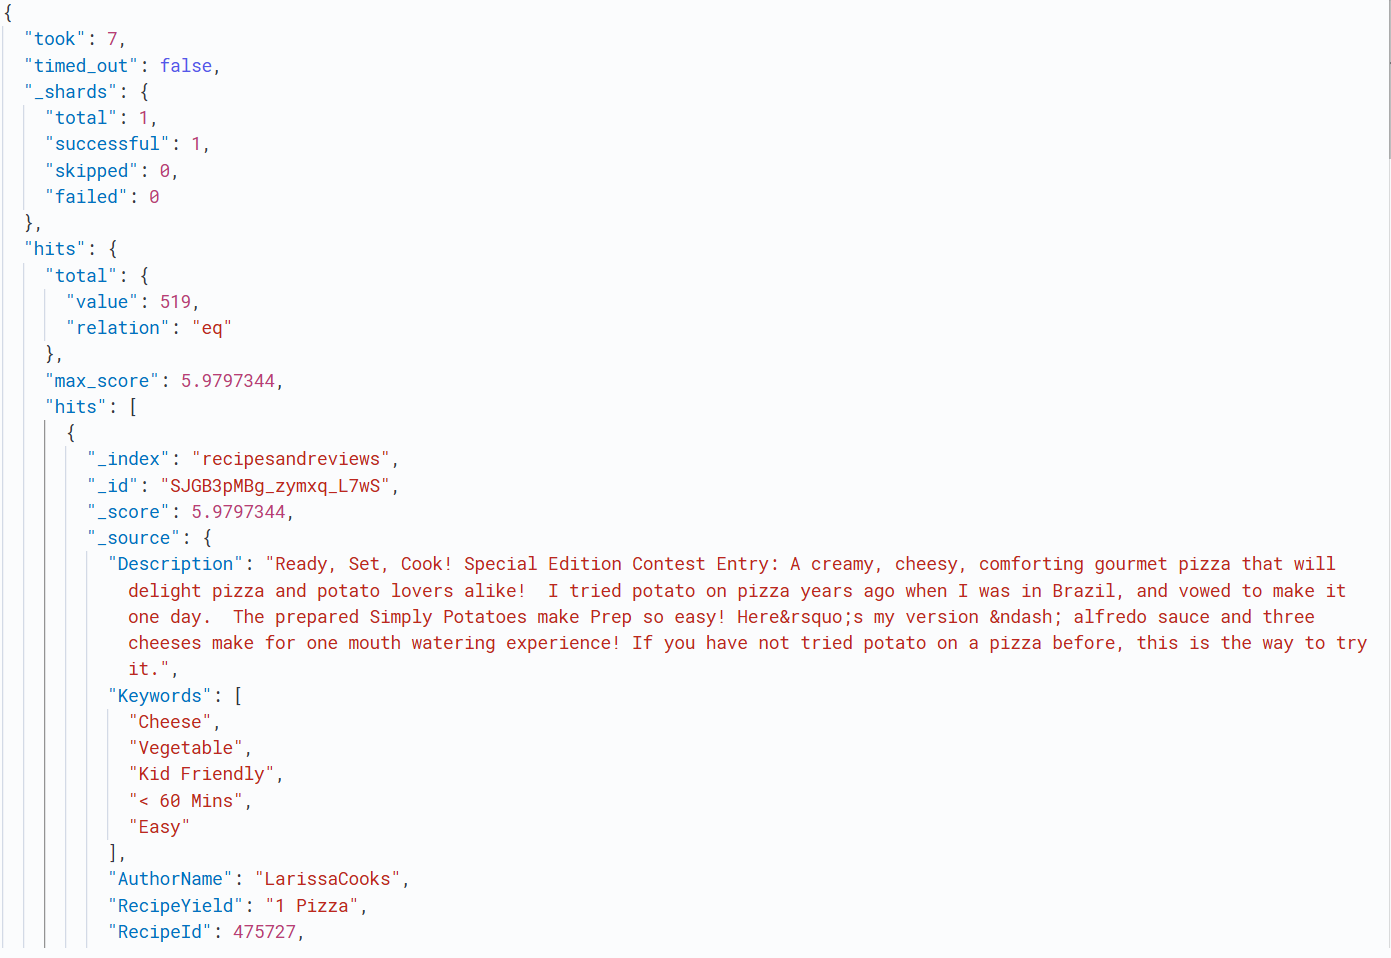
\includegraphics[width=0.8\linewidth]{Report/ReportLatex/Images/ElasticsearchResults/authors1.png}
    \caption{1st result}
    \label{fig:enter-label}
    \end{figure}
    \begin{figure}[H]
    \centering
    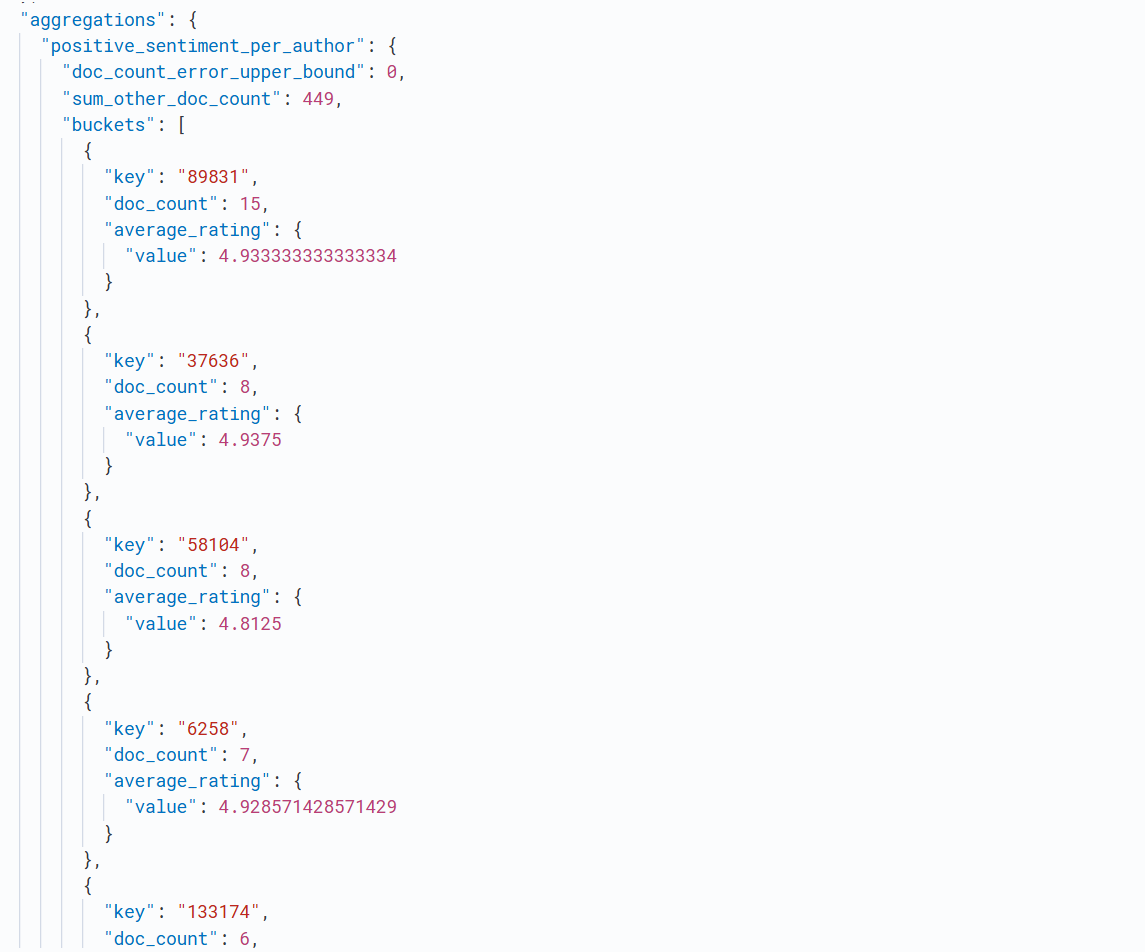
\includegraphics[width=0.8\linewidth]{Report/ReportLatex/Images/ElasticsearchResults/authors2.png}
    \caption{Aggregation output}
    \label{fig:enter-label}
    \end{figure}
    \clearpage
    
    \item \textbf{Easy, budget-friendly recipes ideal for students}

    This query is designed to find recipes that are ideal for college students looking for affordable and easy meal options. The query searches for recipes that are tagged with keywords or descriptions related to "college student," "cheap," and "easy." These terms are used in various fields such as the Description, Keywords, and RecipeCategory to ensure that the results are tailored to the needs of students who are on a budget and looking for simple meal ideas. Additionally, the query looks within Reviews to capture any references to these themes, which helps in identifying recipes that other students have positively reviewed for being cost-effective and easy to prepare.

    To ensure the recipes are practical for busy students, the query includes a must\_not clause that filters out recipes requiring more than 60 minutes of preparation time. This ensures that only quick and efficient recipes are returned, as students often don’t have the luxury of long cooking times. The use of the minimum\_should\_match parameter ensures that the query returns recipes that meet at least one of the keyword or descriptive criteria, providing a diverse set of relevant results.

    \begin{verbatim}
GET /recipesandreviews/_search
{
  "query": {
    "bool": {
      "should": [
          {"match":
            {
              "Description": {
                "query": "college student cheap easy",
                "operator": "or"
              }}},
          {"match":
            {
              "Keywords": {
                "query": " college student cheap easy",
                "operator": "or"
              }}},
          {"match":
            {
              "RecipeCategory": {
                "query": "college student cheap easy",
                "operator": "or"
              }}},
          {"nested":{
          "path": "Reviews",
          "query": {
            "match": {
              "Reviews.Review": {
                "query": "college student cheap easy",
                "operator": "or"
            }}}}}],
      "must_not": [
        {
          "range": {
            "TotalTime": {
              "gte": 60
            }}}],
      "minimum_should_match": 1
    }}}
    \end{verbatim}

    \subsubsection{Result}
    In the pictures below we display the first document returned by the query.
    \begin{figure}[H]
    \centering
    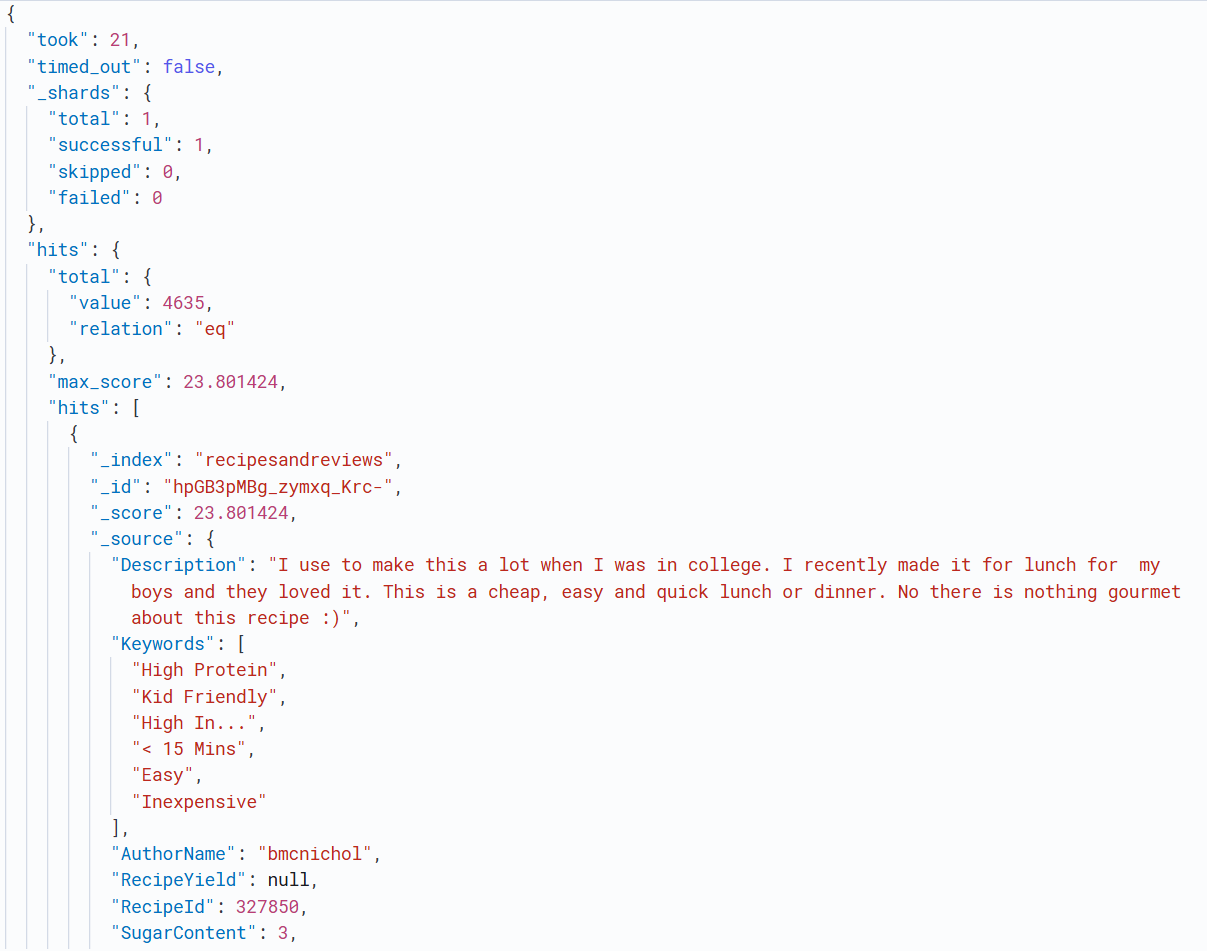
\includegraphics[width=0.7\linewidth]{Report/ReportLatex/Images/ElasticsearchResults/college1.png}
    \caption{1st result (pt.1)}
    \label{fig:enter-label}
    \end{figure}
    \begin{figure}[H]
    \centering
    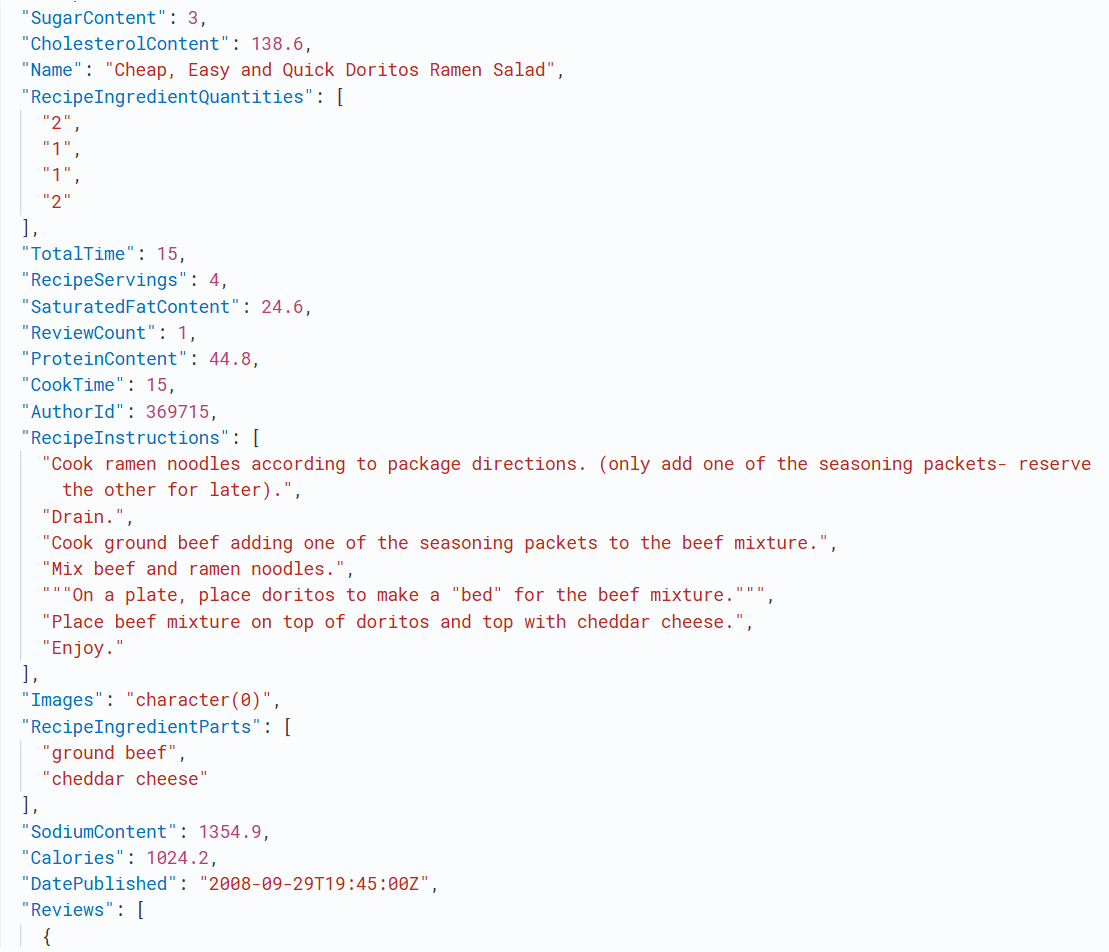
\includegraphics[width=0.7\linewidth]{Report/ReportLatex/Images/ElasticsearchResults/college2.png}
    \caption{1st result (pt.2)}
    \label{fig:enter-label}
    \end{figure}
    \begin{figure}[H]
    \centering
    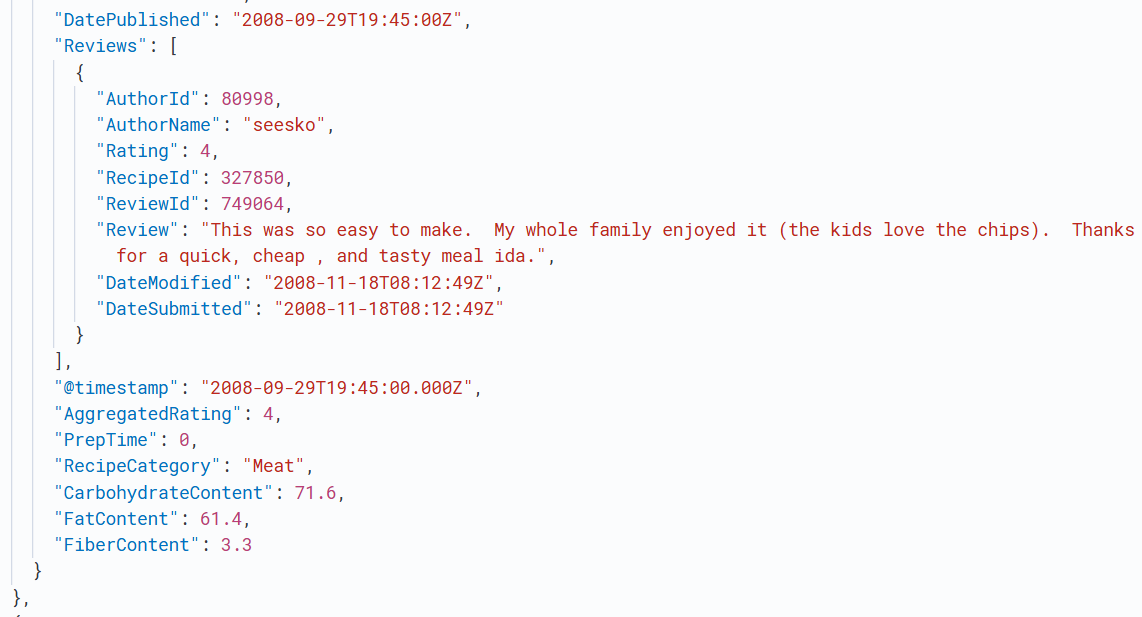
\includegraphics[width=1\linewidth]{Report/ReportLatex/Images/ElasticsearchResults/college3.png}
    \caption{1st result (pt.3)}
    \label{fig:enter-label}
    \end{figure}
\end{enumerate}